\documentclass[notes=hide,8pt,xcolor=svgnames]{beamer}
\usepackage[absolute,overlay]{textpos}
\usetheme[height=7mm]{Madrid}
\usecolortheme[named=MidnightBlue]{structure}
\setbeamertemplate{navigation symbols}{}
\usefonttheme{structurebold}
\usepackage{fancybox}
\usepackage{animate}
\usepackage{amsbsy}

\AtBeginSection[]
{
   \begin{frame}
       \frametitle{Outline}
       \tableofcontents[currentsection]
   \end{frame}
}



% PDF settings
\hypersetup{%
   pdftitle={Energy Preserving Axisymmetric Finite Elements for Lagrangian Hydrodynamics},%
   pdfauthor={Truman E. Ellis},%
   pdfsubject={Finite Element, Lagrangian Hydrodynamics, Axisymmetry, Energy Conserving, Symmetry Preserving},%
   pdfkeywords={Finite Element, Lagrangian Hydrodynamics, Axisymmetry, Energy Conserving, Symmetry Preserving}%
}

\setlength{\TPHorizModule}{0.1\textwidth}
\setlength{\TPVertModule}{0.1\textheight}


\title[Energy Preserving r-z FEM for Lag. Hydro]{\LARGE Energy Preserving Axisymmetric Finite Elements for Lagrangian Hydrodynamics}
\author[Truman Ellis]{{\Large Truman E. Ellis}\\[1ex]
{\small Joint work with: Veselin Dobrev (CASC), Tzanio Kolev* (CASC), and Robert Rieben* (WCI)}\\
{\small *Mentors}}
\institute[ISCR]{\footnotesize
  Institute for Scientific Computing Research\\
  Lawrence Livermore National Laboratory\\
  Livermore, CA 94550\\[1ex]
  \texttt{ellis35@llnl.gov}
}
\date[August 2010]{August 3, 2010}

\begin{document}

\begin{frame}[plain]
  \titlepage
  \begin{center}
  \vskip-8ex
   
\includegraphics[height=0.5in]{figures/LLNL_logo.png}
  \end{center}
  \begin{textblock}{8}[0.5,0.5](5,10.5)
  \centering
  \color{blue}{\tiny This work performed under the auspices
      of the U.S. Department of Energy by
      Lawrence Livermore National Laboratory

      under Contract DE-AC52-07NA27344
      LLNL-PRES-445911
      }
  \end{textblock}
%   \begin{textblock}{8}[0.5,0.5](12.5,10.8)
%    \tiny{\rmfamily Powered by \LaTeX}
%   \end{textblock}
\end{frame}

\begin{frame}
\frametitle{Introduction}
\begin{columns}
\begin{column}{0.55\textwidth}
Our goal is to improve the traditional staggered grid hydro (SGH) algorithms used to solve the Euler equations in multi-material ALE codes with respect to:
\begin{itemize}
   \item Mesh imprinting / instabilities
   \item \textbf<2>{\textcolor<2>{LimeGreen}{Symmetry preservation}}
   \item \textbf<2>{\textcolor<2>{LimeGreen}{Total energy conservation}}
   \item Artificial viscosity
\end{itemize}

\medskip
We consider a new approach\footnote[frame,1]{\tiny V. Dobrev, T. Ellis, Tz. Kolev, R. Rieben, "Curvilinear finite elements for Lagrangian hydrodynamics". IJNMF, to appear} based on a generalized FEM treatment of the Euler equations in a Lagrangian frame with the following features:

\begin{itemize}
   \item Curvilinear zone geometries
   \item Higher order field representations
   \item \textbf<2>{\textcolor<2>{LimeGreen}{Exact discrete energy conservation by construction}}
   \item Reduces to classical SGH under simplifying assumptions
   \item Can be viewed as a high order extension of SGH
\end{itemize}
\end{column}
\begin{column}{0.45\textwidth}
\begin{center}
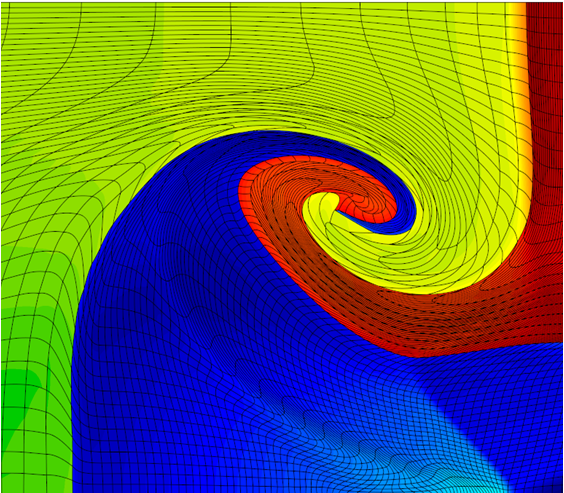
\includegraphics[width=1\textwidth]{figures/IntroTriplePoint.png}
Curvilinear FEM Lagrangian calculation of shock triple point interaction.
\end{center}
\end{column}
\end{columns}
\end{frame}
\note{
This is my third summer working on this project. Our goal is to improve the traditional staggered grid hydro (SGH) algorithms used to solve the Euler equations in multi-material ALE codes with respect to
\begin{itemize}
\item mesh imprinting and mesh instabilities \\
(i.e. problems with shock-mesh interaction and hourglass modes)
\item symmetry preservation \\
(that is problems which should conserve symmetry, but don't with our current numerical methods)
\item total energy conservation \\
(traditional methods do not conserve energy in cylindrical coordinate systems)
\item artificial viscosity discretization
\end{itemize}

\medskip
We have developed a general high order FEM discretization of the Euler equations in a Lagrangian frame that
\begin{itemize}
\item allows for curvilinear zone geometries \\
(which improves the robustness of Lagrangian simulations)
\item exactly conserves energy by construction
\item is a direct higher order extension of classical SGH
\end{itemize}

\medskip
My research this summer has focused on extending our method to axisymmetric problems. In so doing, we will be addressing the issues of symmetry preservation and energy conservation.
}


\begin{frame}
 \frametitle{Outline}
 \tableofcontents
\end{frame}

\note{
But before we can address axisymmetry we have to cover some basics. \\
\begin{itemize}
\item Physically, what are we solving? What are hydrodynamics? \\[2ex]
\item And what specifically are Lagrangian hydrodynamics? \\[2ex]
\item Before we can We will be extending our method from Cartesian to cylindrical coordinates, \\
so we first need to establish our method in a x-y-z coordinate system.
\end{itemize}

\medskip
Then we will be ready to examine the necessary additions to consider axisymmetric problems.\\
Finally, we will consider a slew of different numerical problems designed to stress
test our new axisymmetric hydrocode.
}

\section{Introduction}
\subsection{Euler Equations}


% Euler Equations in Lagrangian Frame
\begin{frame}
  \frametitle{Euler Equations in a Lagrangian Frame}
\begin{columns}
\begin{column}{0.6\textwidth}
\begin{block}<+->{\small The Euler equations of gas dynamics in a Lagrangian reference
frame can be written in differential form as:}
\bigskip

\begin{tabular}{ll}
Momentum Conservation: & $\rho \dfrac{\mathrm{d} \vec v}{\mathrm{d} t}=-\nabla p +...$\\ \\
Mass Conservation: & $\dfrac{1}{\rho}\dfrac{\mathrm{d} \rho}{\mathrm{d} t}=-\nabla\cdot \vec{v} $ \\ \\
Energy Conservation: & $\rho \dfrac{\mathrm{d} e}{\mathrm{d} t} =-p\nabla\cdot \vec{v} +...$ \\ \\
Equation of State: \medskip& $p=EOS(e, \rho)$ \\
Equation of Motion: & $\dfrac{\mathrm{d}\vec x}{\mathrm{d}t}=\vec{v}$ \\
\end{tabular}
\end{block}
\vskip3em
\end{column}
\begin{column}{0.35\textwidth}
\small
Typically, these equations are solved on a staggered spatial grid \footnote[frame,1]{\tiny R. Tipton, ``CALE Lagrange Step”, unpublished LLNL report, 1990}$^,$\footnote[frame,2]{\tiny M. Wilkins, ``Calculations of Elastic-Plastic Flow,” Methods of Computational Physics, 1964}
where thermodynamic variables are approximated as piece-wise constants defined on zone centers and kinematic variables are defined on the nodes.

\medskip
Spatial gradients are computed using finite volume and/or finite difference methods:
\begin{center}
 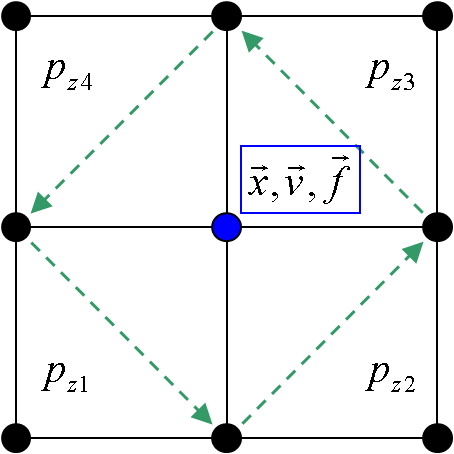
\includegraphics[width=0.85\textwidth,keepaspectratio=true]{figures/HEMPLagHydro.png}
\end{center}
\end{column}
\end{columns}
\end{frame}

\note{
The Euler equations are a simplfied form of the Navier-Stokes equations of fluid
motion in which we assume that inertial forces are much more significant than
viscous forces. This allows us to assume all of the complicated viscous terms are
negligible, and we are left with the following simplified system of equations.\\
\medskip

We have our traditional conservation of momentum, mass, and energy. Then we have
our equation of state which is a material property and can be a function, lookup
table, etc. And finally, we have our simple equation of motion. \\
\medskip

Traditionally these have been solved on a staggered spatial grid where the
thermodynamic variables of density, energy, and pressure are represented as
piecewise constant values defined at cell centers and the kinematic variables of
position and velocity are define at the mesh nodes. The spatial gradients in
these equations have typically been solved with either finite difference or
finite volume methods.
}

\subsection{Lagrangian Mesh Motion}


\begin{frame}
 \frametitle{Lagrangian Mesh Motion}
 \begin{columns}[T]
  \begin{column}{0.6\textwidth}
   After deformation in time, zones are reconstructed based on particle locations, thus defining the moved mesh.
   \begin{columns}[b]
   \begin{column}{0.5\textwidth}
   \begin{figure}[h!]
    \centering
    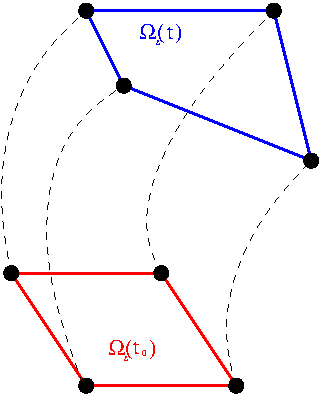
\includegraphics[width=0.9\textwidth,keepaspectratio=true]{figures/Motion-Q1.pdf}
    \end{figure}
    \parbox{0.8\textwidth}{\centering \small
    Q1 (Bi-Linear) Approximation}
    \end{column}
    \begin{column}{0.5\textwidth}
    \begin{figure}[h!]
    \centering
    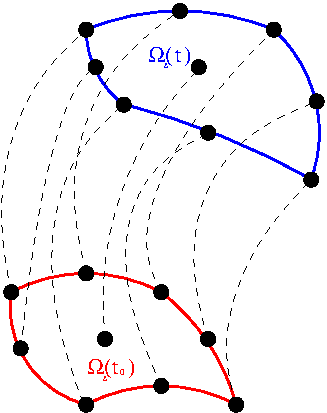
\includegraphics[width=0.9\textwidth,keepaspectratio=true]{figures/Motion-Q2.pdf}
    \end{figure}
    \parbox{0.8\textwidth}{\centering \small
    Q2 (Bi-Quadratic) Approximation}
    \end{column}
    \end{columns}
  \end{column}
  \begin{column}{0.35\textwidth}

   This reconstruction process has an inherent geometric error.
   \begin{block}{}
    \begin{figure}[h!]
    \centering
    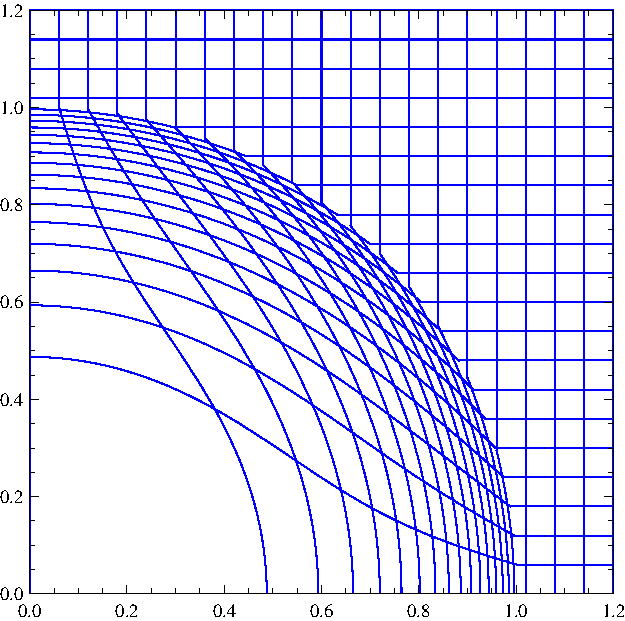
\includegraphics[width=1.0\textwidth,keepaspectratio=true]{figures/Motion-Sedov.pdf}
    \end{figure}
    \vskip-2ex
    \small
    Initial Cartesian mesh deformed with the exact solution of the Sedov blast wave problem.
   \end{block}
  \end{column}
 \end{columns}
 \begin{block}{}
 \small
 High order finite elements that use additional particle degrees of freedom are
 able to more accurately represent continuous deformations.
 \end{block}
\end{frame}

\note{
In a Lagrangian simulation, the mesh moves with the material. The mesh is
defined by its nodes, thus at each time step we move these nodes as if they were
particles in the flow. Then we reconstruct our mesh based on the updated particle
locations. \\ \medskip

In 2D, a bi-linear zone is defined by a set of 4 vertices that move in time. We
can reconstruct these zones by drawing straight lined edges between the vertices.
Alternatively we can define higher order bi-quadratic, bi-cubic, or higher order
zones. Bi-quadratic zones are defined by 9 nodes which can be connected with
quadratic edges which can result in curvilinear elements. \\ \medskip

No matter what kind of elements we choose, there will always be some level of
error inherent in this reconstruction process. For example, consider the Sedov
blast problem. If we take an initially Cartesian mesh and continuously deform
all of the mesh edges according the exact solution to the Sedov problem, we get
the curvilinear mesh on the right. \\ \medskip

High order finite elements that use additional particle degrees of freedom are
able to more accurately represent continuous deformations.
}


\section{Cartesian Theory}
\note{
Now that we've established our problem, we need to develop the Cartesian version
of our method before we can extend it to axisymmetric problems.
}
\subsection{Kinematics}


\begin{frame}[fragile]
\frametitle{Kinematics}
\small
 Velocity and position are approximated with high order finite elements using
basis functions $\vec w_i$:
$$
\vec{v}(\vec{x},t)\approx \displaystyle\sum_i^{N_v} \mathbf{v}_i(t) \vec w_i(\vec{x})
$$
\begin{center}
\begin{minipage}{0.7\textwidth}
 \begin{columns}
  \begin{column}{0.3\textwidth}
  \centering
  \small
  \textcolor{red}{\underline{Reference Space:}}
    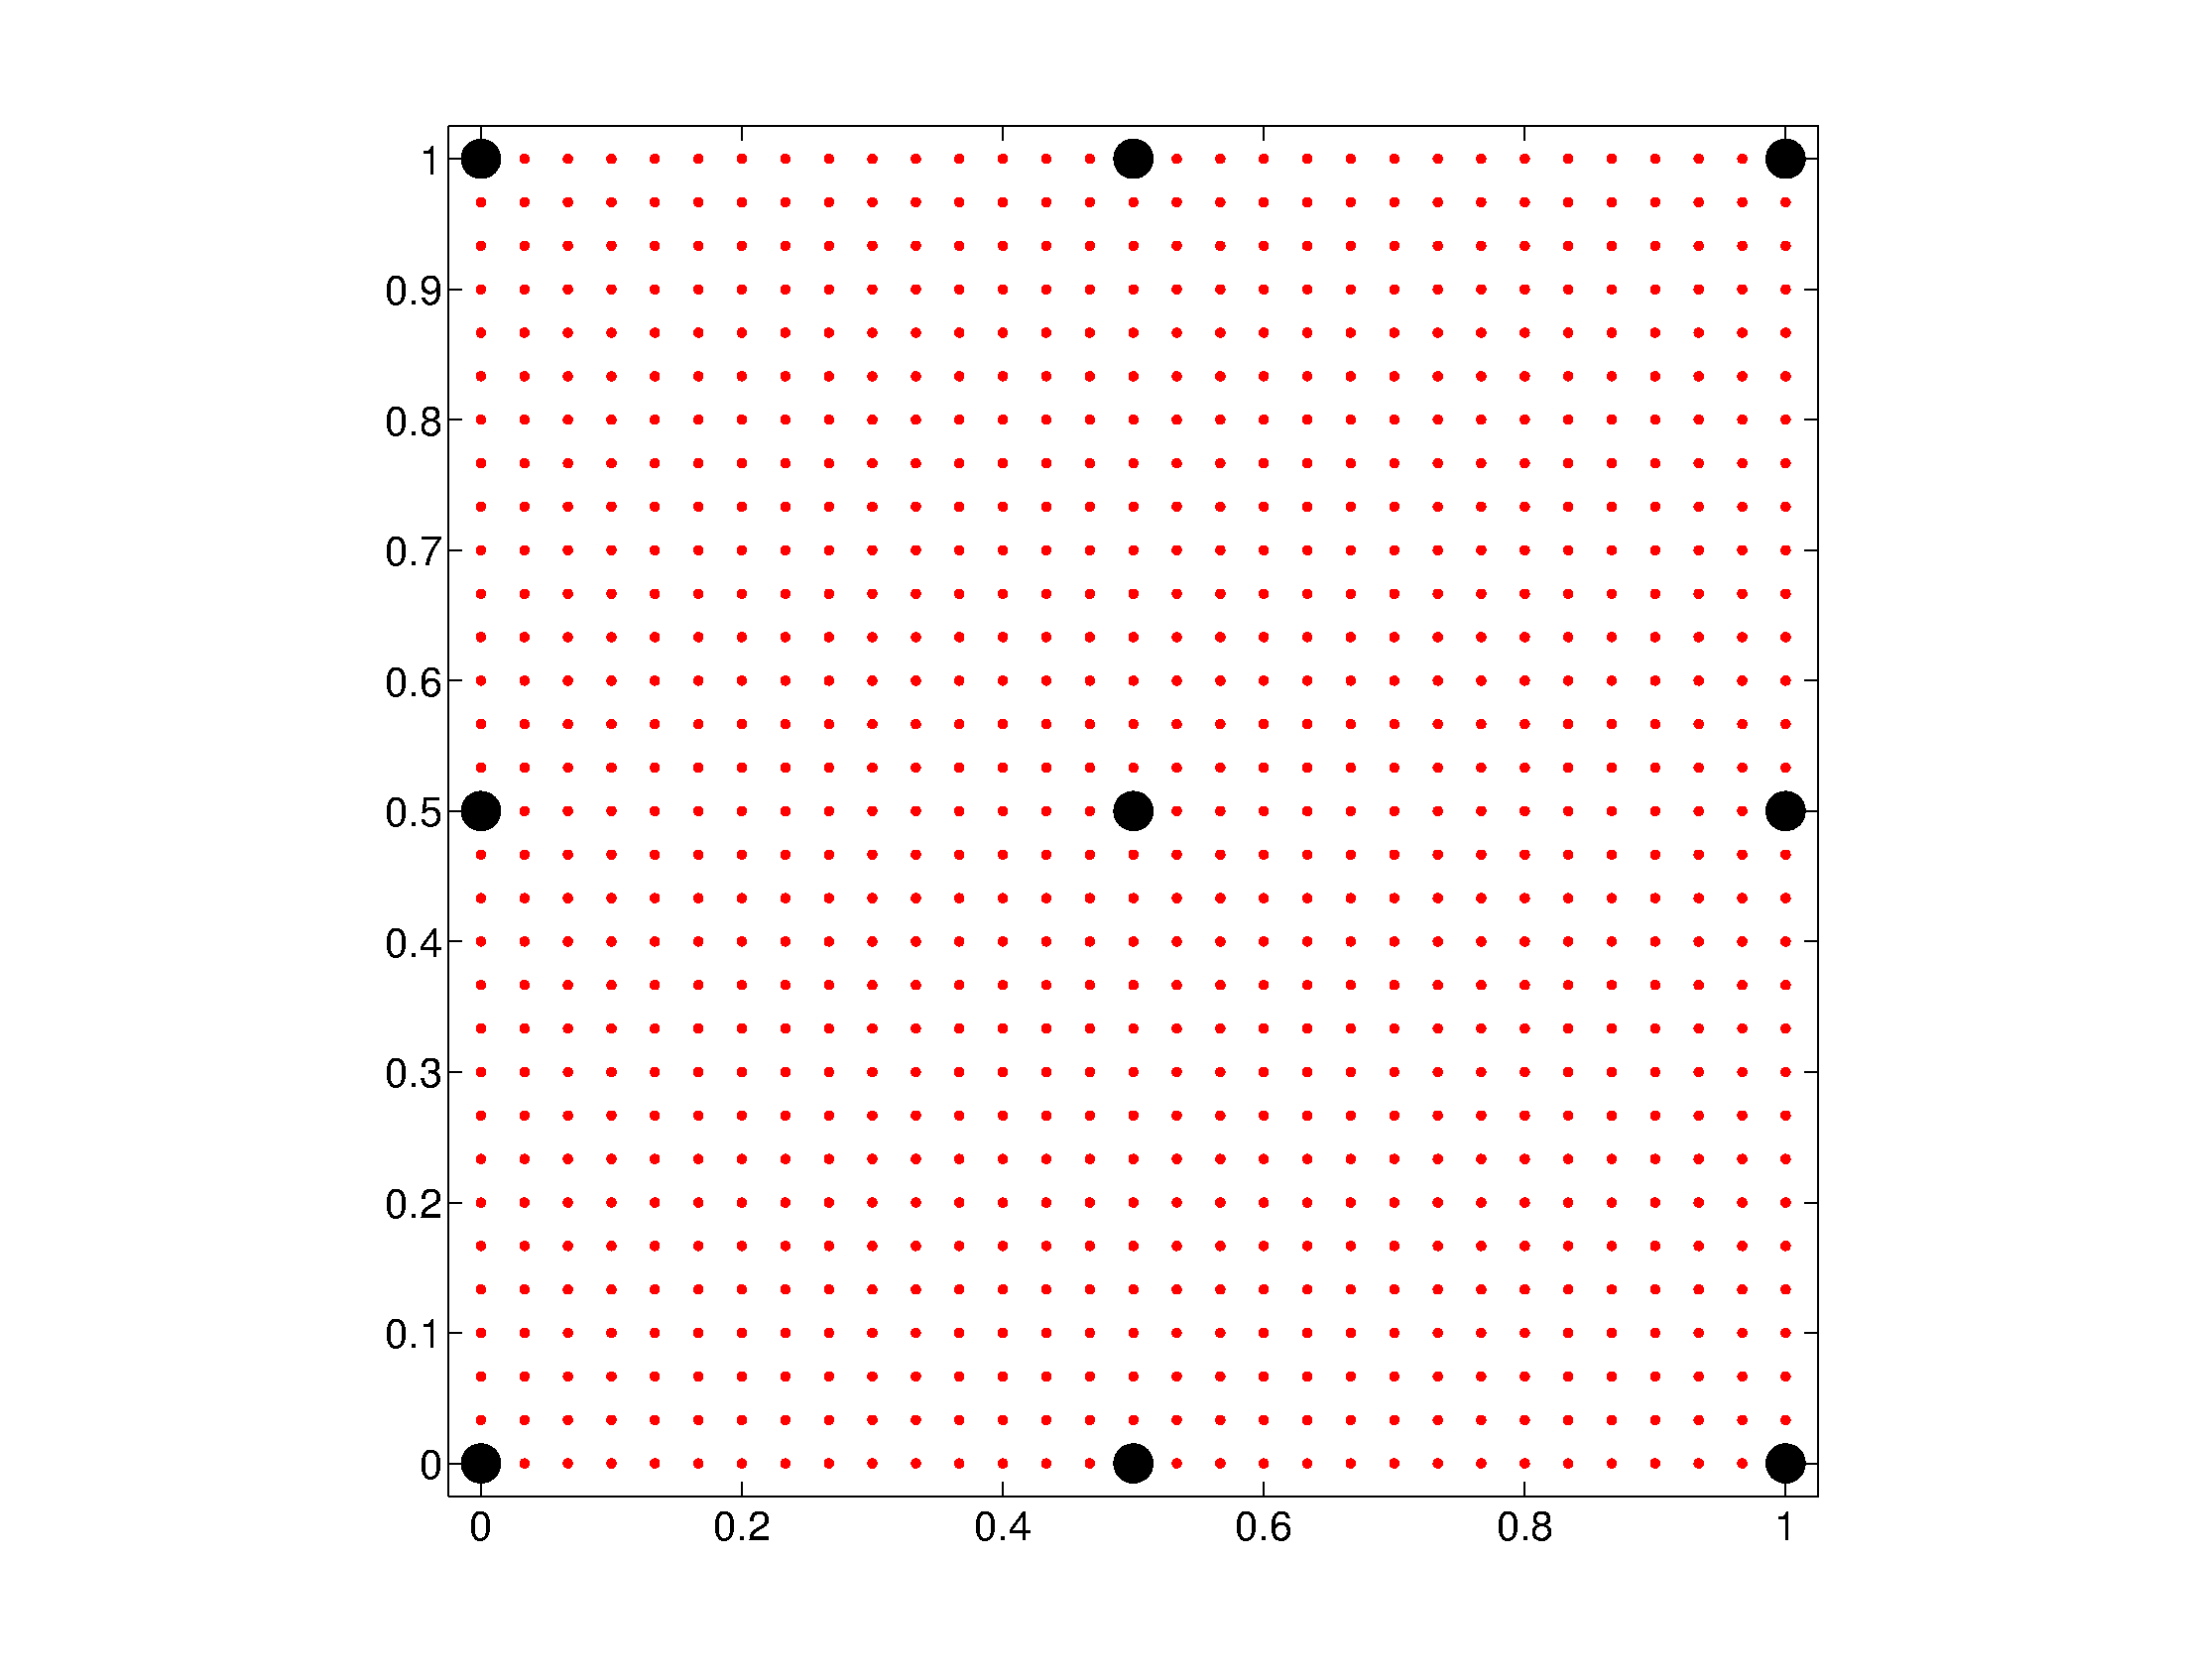
\includegraphics[width=1.0\textwidth,keepaspectratio=true,viewport=200 50
900 775]{figures/Q2_Element_Ref.pdf}
%     \textcolor{red}{$\phi(\hat{\vec{x}})$} \\[1ex]
%     \textcolor{red}{$\vec{\nabla}\phi(\hat{\vec{x}})$}
  \end{column}
  \begin{column}{0.2\textwidth}
   \begin{figure}[h!]
    \centering
    \vskip-5ex
    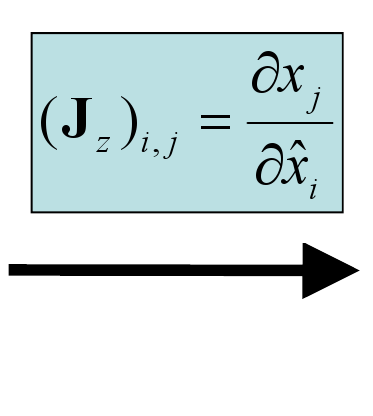
\includegraphics[width=1.0\textwidth,keepaspectratio=true]{figures/transSpace_new.png}
    \end{figure}
  \end{column}
  \begin{column}{0.3\textwidth}
  \centering
  \small
  \textcolor{blue}{\underline{Physical Space:}}
    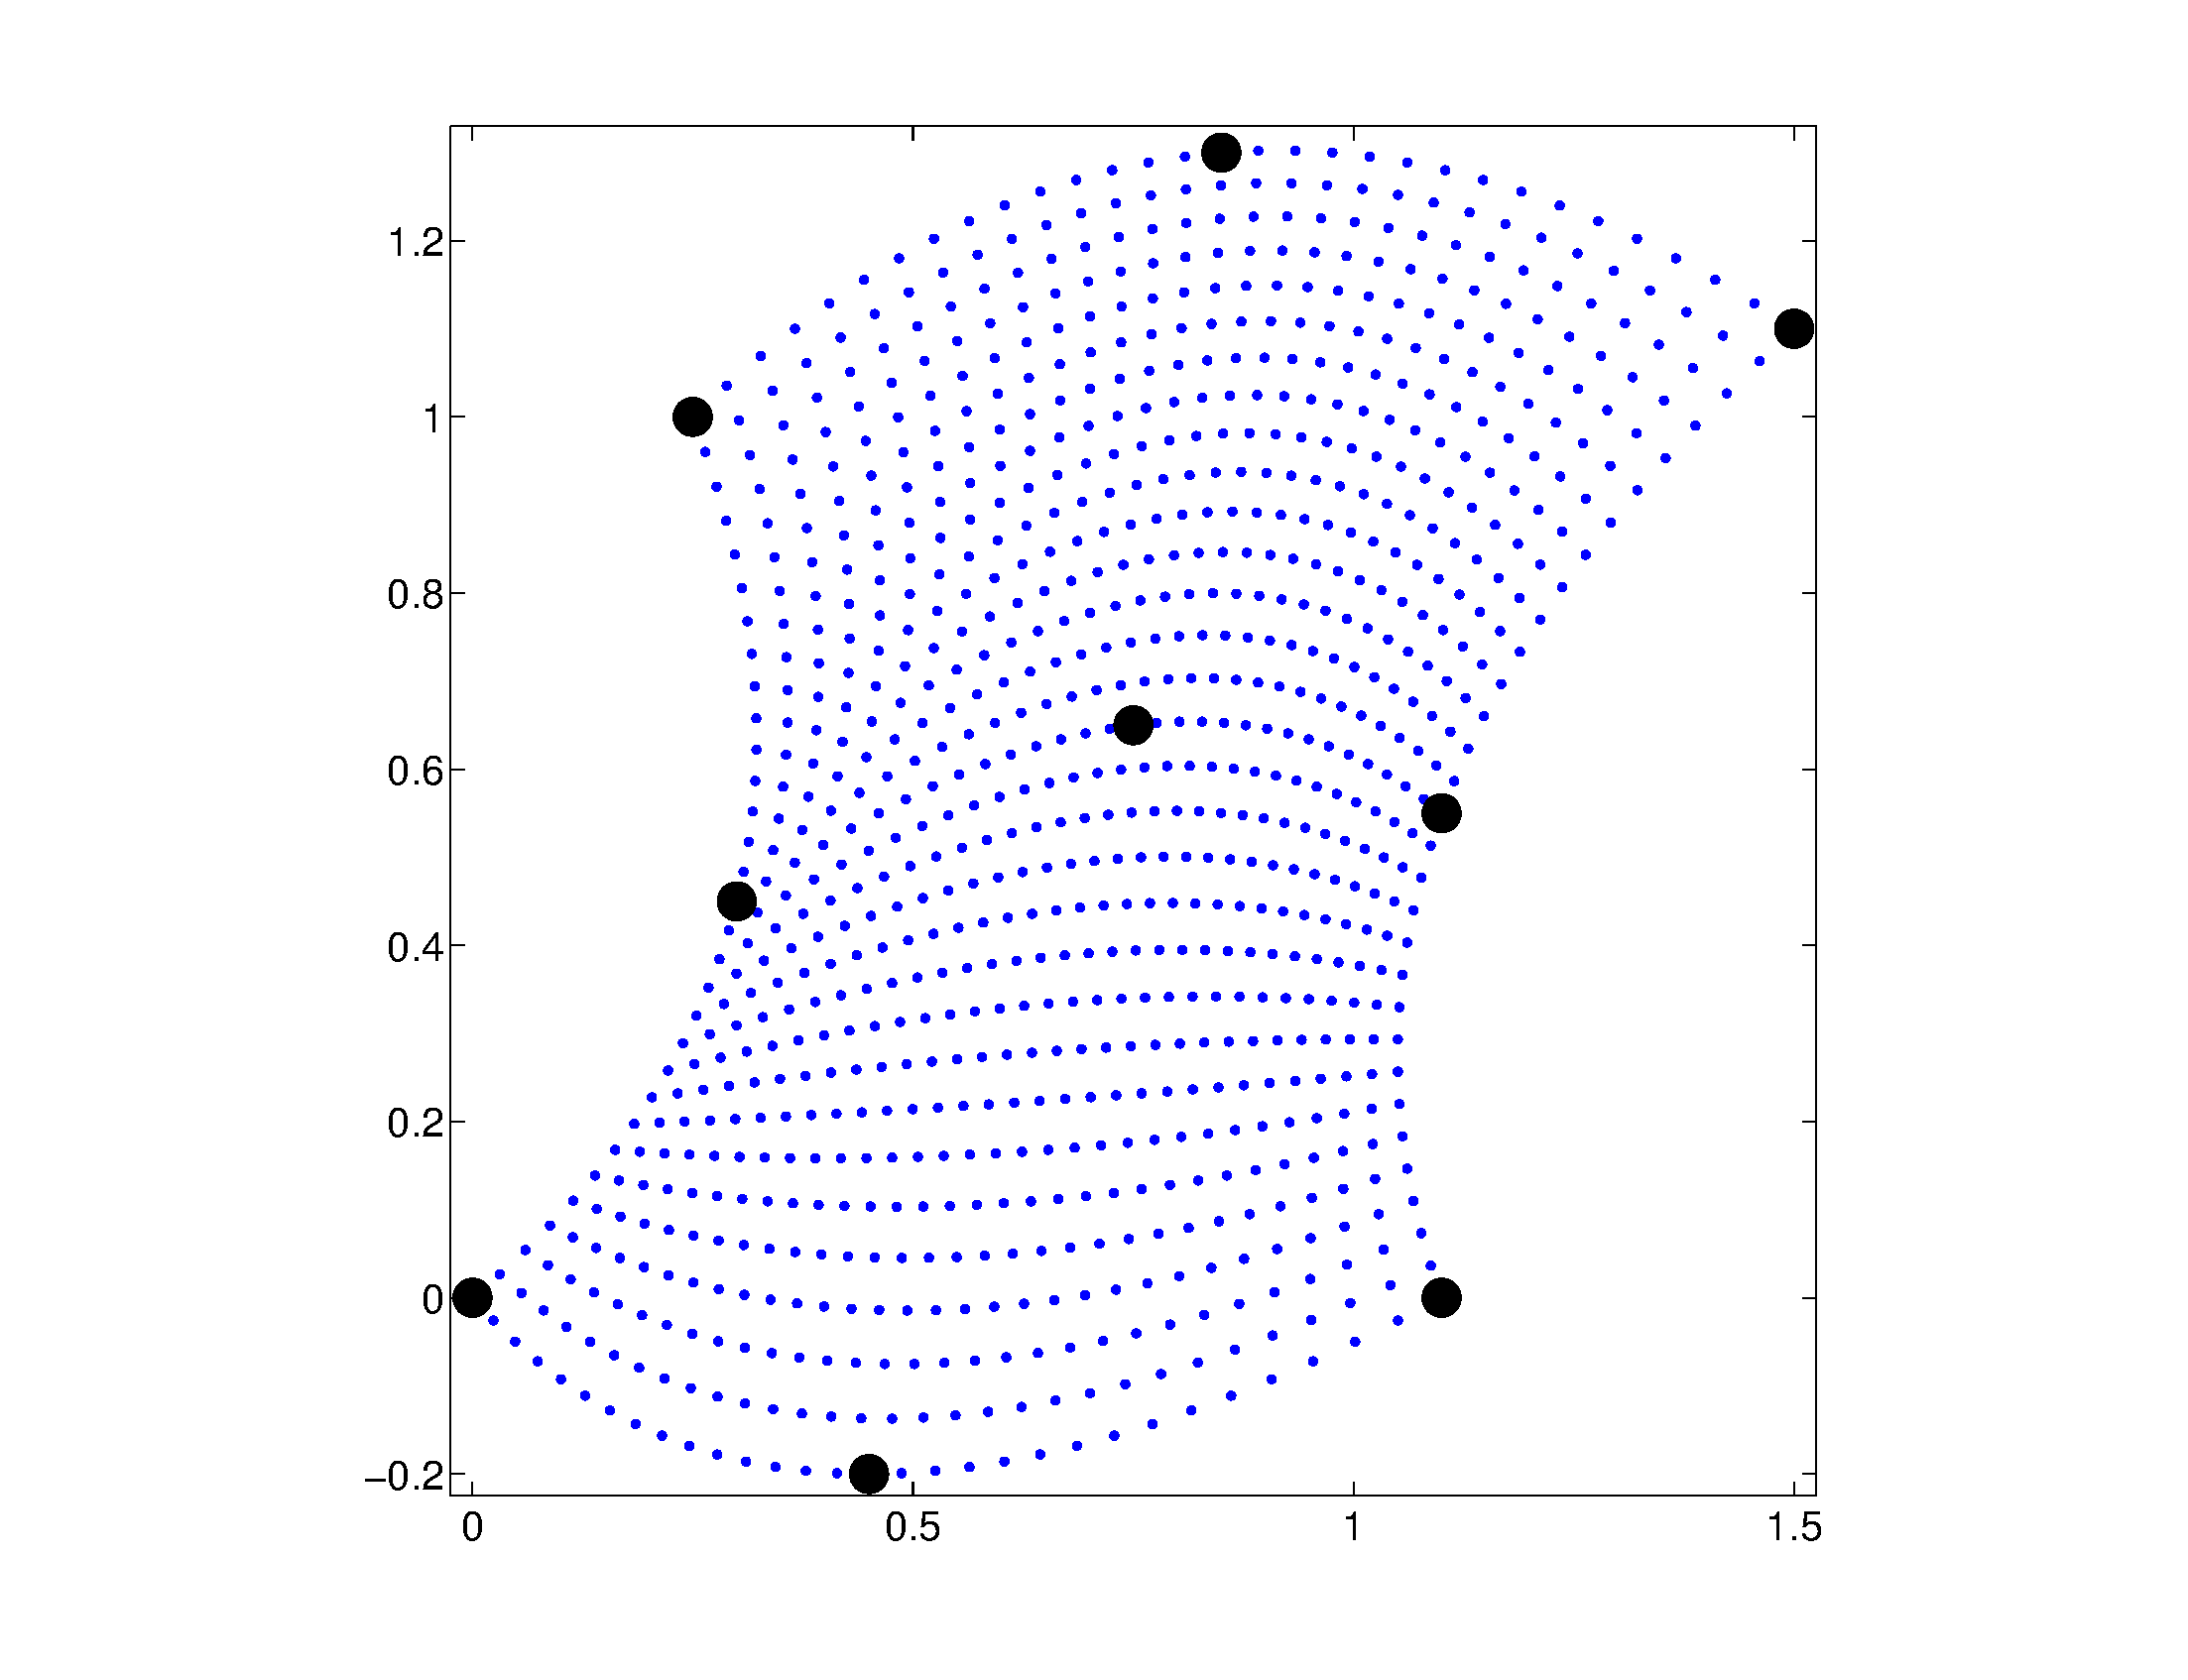
\includegraphics[width=1.0\textwidth,keepaspectratio=true,viewport=200 50
900 775]{figures/Q2_Element_Phys.pdf}
%     \textcolor{blue}{$\phi(\vec{x})=\hat{\phi}(\Phi^{-1}(\vec{x}))$} \\[1ex]
%     \textcolor{blue}{$\vec{\nabla}\phi=J_Z^{-1}\vec{\nabla}\hat{\phi}$}
  \end{column}
 \end{columns}
 \end{minipage}
 \end{center}
{\small The Position DOFs define the mapping from a reference element to physical space.} %The derivative of this mapping is the Jacobian matrix}

\medskip
Weak formulation of the momentum conservation equation with a tensor artificial viscosity\footnote[frame,1]{\tiny Tz. Kolev, R. Rieben, "A tensor artificial viscosity using a finite element approach", Journal of Computational Physics 2009}:
\[
\int_{\Omega(t)} \left(\rho\dfrac{\mathrm{d}\vec{v}}{\mathrm{d}t}\right)\cdot \vec{w}_i
 =\int_{\Omega(t)} (-\nabla p +\nabla \cdot \mu\nabla\vec{v}) \cdot \vec{w}_i
 =\int_{\Omega(t)} (p\mathbf{I}-\mu\nabla\vec{v}) :\nabla\vec{w}_i
\]
\vskip-1.5ex
\begin{columns}[T]
\begin{column}{0.2\textwidth}
\begin{block}{Velocity Mass Matrix}
\centering
$\displaystyle
\mathbf{M}_v=\int_{\Omega}\rho \mathbf{w} \mathbf{w}^T
$
\end{block}
\end{column}
\begin{column}{0.15\textwidth}
\begin{block}{Stress Tensor}
\vskip1.5ex
\centering
$\displaystyle
\sigma = -p\mathbf{I}+\mu\nabla\vec{v}
$
\vspace{-.5ex}
\end{block}
\end{column}
\begin{column}{0.28\textwidth}
\begin{block}{Conservation of Momentum}
\centering
$\displaystyle
\mathbf{M}_v \frac{\mathrm{d}\mathbf{v}}{\mathrm{d}t}=-\int_{\Omega}\sigma: \nabla \mathbf{w}
$
\end{block}
\end{column}
\begin{column}{0.18\textwidth}
\begin{block}{Equation of Motion}
\centering
$\displaystyle
\frac{\mathrm{d}\mathbf{x}}{\mathrm{d}t}=\mathbf{v}
$
\vspace{.4ex}
\end{block}
\end{column}
\end{columns}
\smallskip
\end{frame}

\note{
We can use the set of basis functions, $w_i$ to represent our kinematic variables
in a basis function expansion.\\ \medskip

The position DOFs in each zone define the mapping from a reference unit square
to the physical element that we are modeling. \\ \medskip

At each timestep we need to know the velocity at each position DOF so we
can move them to the correct location. Solving the momentum equation, $F=m a$
gives us these new velocities and the equation of motion gives us the new
positions. On the left hand side of the momentum equation we have $m a$, the
integral of density multiplied by the time derivative of velocity. And on the
right hand side we have $F$, the integral of the stress. \\ \medskip

We can write our momentum equation in FEM-ready weak form by
mulitiplying both sides by a test function and integrating by parts. In the
resulting system of equations, we equate the velocity mass matrix time the time
derivative of velocity with the integral of the stress tensor $\sigma$ \\ \medskip

Also, please note our notation conventions. An arrow represents a physical
vector field, bold face a linear algebra object, lower case for an array, upper
case for a matrix.
}


\subsection{Thermodynamics}


\begin{frame}
\frametitle{Thermodynamics}
\small
Internal energy is approximated from the set of discontinuous basis functions $\phi_i$:
\[
e(\vec{x},t)\approx \displaystyle\sum_i^{N_e} \mathbf{e}_i(t) \phi_i(\vec{x})
\]
\vskip-3ex
\begin{columns}
\begin{column}{0.2\textwidth}
\centering
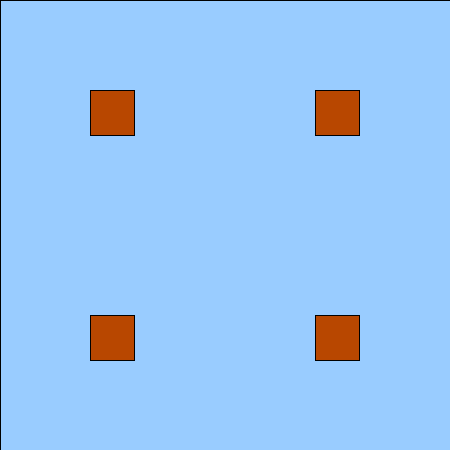
\includegraphics[width=0.8\textwidth]{figures/Thermo_DOFs.pdf} \\
Internal energy DOFs on reference element
\end{column}
\begin{column}{0.3\textwidth}
\centering
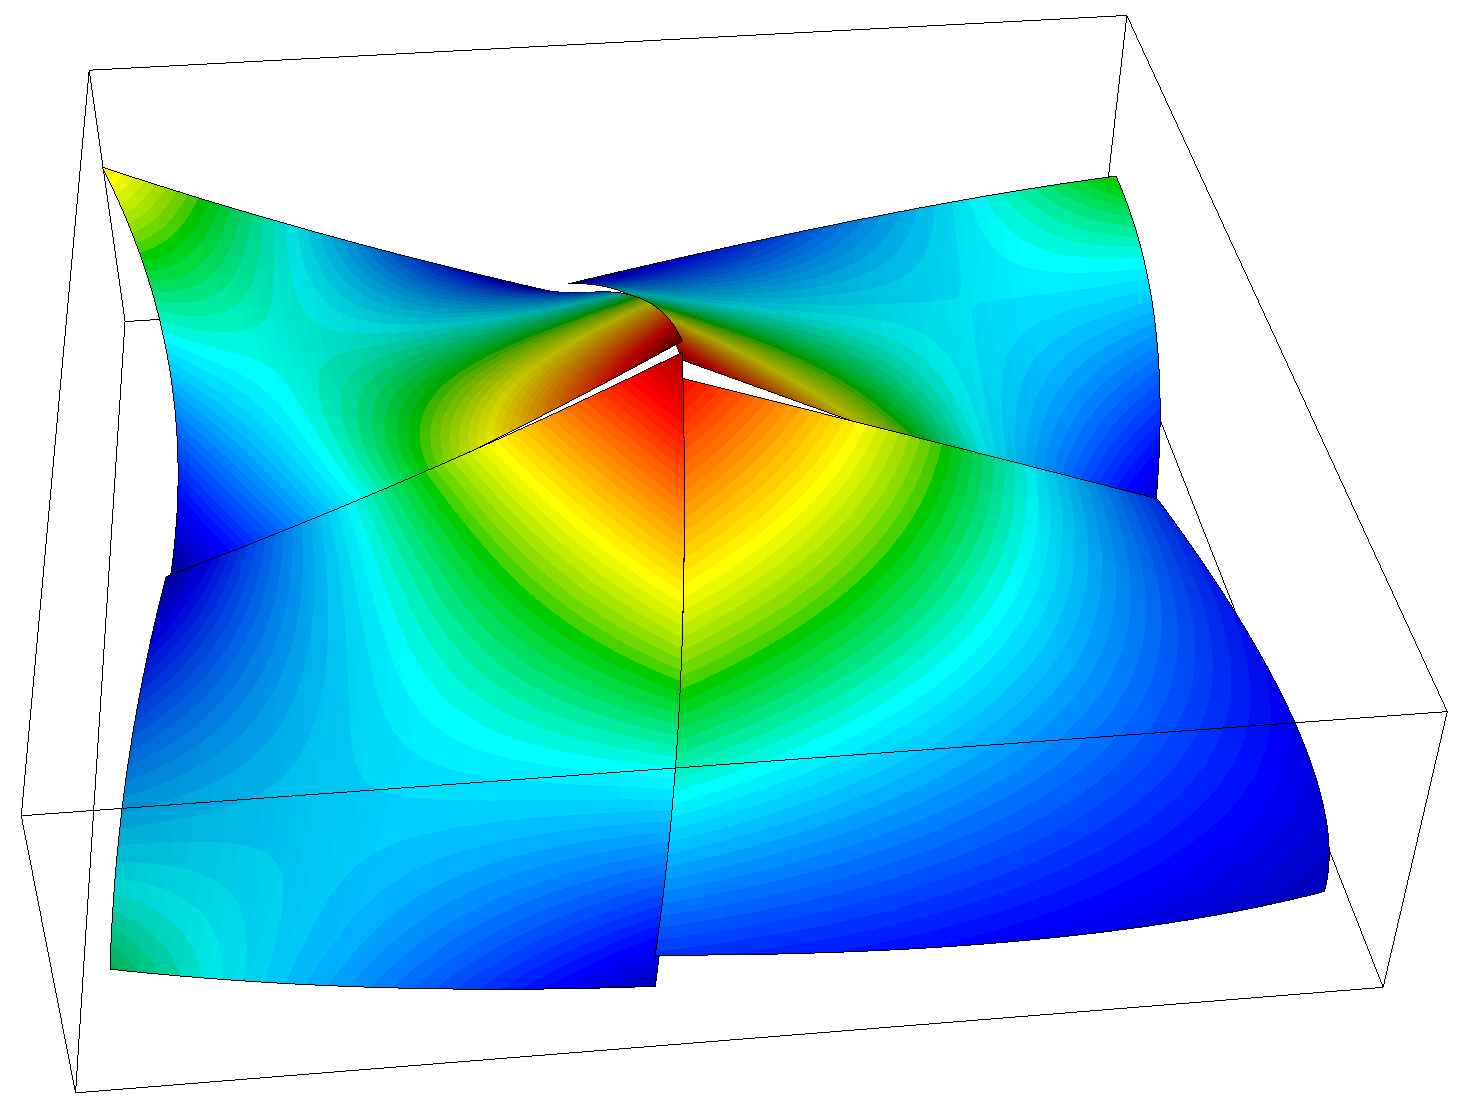
\includegraphics[width=0.8\textwidth]{figures/disc_field.png} \\
Patch of discontinuous $Q_1$ elements
\end{column}
\end{columns}
\medskip
Weak formulation of the energy conservation equation on zonal level
\[
\int_{\Omega_z(t)} \left(\rho\dfrac{\mathrm{d}e}{\mathrm{d}t}\right) \phi_i
 =\int_{\Omega_z(t)} (\sigma :\nabla\vec{v}) \, \phi_i
 \]
\begin{columns}
\begin{column}{0.3\textwidth}
\begin{block}{Energy Mass Matrix}
\centering
$\displaystyle
\mathbf{M}_{e}=\int_{\Omega}\rho \boldsymbol{\phi} \boldsymbol{\phi}^T
$
\end{block}
\end{column}
\begin{column}{0.3\textwidth}
\begin{block}{Conservation of Energy}
\centering
$\displaystyle
\mathbf{M}_{e} \frac{\mathrm{d}\mathbf{e}}{\mathrm{d}t}=\int_\Omega (\sigma : \nabla \vec{v}) \, \boldsymbol{\phi}
$
\end{block}
\end{column}
\end{columns}
\medskip

Since the FEM space is discontinuous, $\mathbf{M}_{e}$ is block-diagonal and
the above equation reduces to separate equations local to each zone.
\end{frame}

\note{
We can use the set of discontinuous basis functions, $\phi_i$ to represent
internal energy in a basis function expansion.\\ \medskip

The IE DOFs are independent of surrounding cells, thus in general we can get
discontinuous thermodynamic fields. \\ \medskip

Here we have the weak form of the energy conservation equation. Similar to
momentum conservation, we have an energy mass matrix and a right hand side which
include the stress tensor.

Since the FEM space is discontinuous, $\mathbf{M}_{e}$ is block-diagonal and
this equation reduces to separate equations local to each zone.
}


\subsection{Conservation of Mass}


\begin{frame}
\frametitle{Mass Conservation}
\begin{center}
\Ovalbox{
\begin{minipage}[c]{0.45\textwidth}
In the Lagrangian description, the total mass of a zone is constant for all time:
\end{minipage}
\begin{minipage}[c]{0.4\textwidth}
\[
\frac{\mathrm{d}m_z}{\mathrm{d}t}=0,\quad m_z=\int_{\Omega_z(t)}\rho
\]
\end{minipage}
}
\end{center}
\begin{columns}[T]
\begin{column}{0.45\textwidth}
\begin{block}{Weak Formulation}
\centering
We define high order zonal mass moments:

\smallskip
$\displaystyle
\mathbf{m}_{z,i}\equiv \int_{\Omega_z(t)}\rho\phi_i
$

\smallskip
Inserting the basis function expansion for density and writing in matrix vector form:
\smallskip

$\displaystyle
\mathbf{m}_z=\mathbf{M}_z^\rho\boldsymbol{\rho}_z
$ where
$\displaystyle
\left(\mathbf{M}_z^\rho\right)_{i,j}\equiv\int_{\Omega_z(t)}\phi_i\phi_j
$

\medskip
We therefore generalize zonal mass conservation to the high order moments:

\smallskip
\fcolorbox{black}{cyan!30}{
$\displaystyle
\frac{\mathrm{d}}{\mathrm{d}t}\left(\mathbf{M}_z^\rho\boldsymbol{\rho}_z\right)=0
$}
\end{block}
\end{column}
\begin{column}{0.45\textwidth}
\begin{alertblock}{Strong Formulation}
\centering
If we impose the stronger condition:

\smallskip
$\displaystyle
\frac{\mathrm{d}}{\mathrm{d}t}\int_{\Omega_z(t)}\rho\psi=0\quad
$
for \textbf{any} function $\psi$

\medskip
then we obtain the
\mbox{\alert{strong mass conservation principle:}}
\medskip

\fcolorbox{black}{cyan!30}{
$\displaystyle
\rho(t)|\mathbf{J}(t)|=\rho(t_0)|\mathbf{J}(t_0)|
$}

\medskip
Furthermore, this implies that the mass matrices are constant for all time:
\vskip-2.3ex
\[
\frac{\mathrm{d}\mathbf{M}_v}{\mathrm{d}t}=0, \quad
\frac{\mathrm{d}\mathbf{M}_e}{\mathrm{d}t}=0
\]
\end{alertblock}
\end{column}
\end{columns}
\medskip
\begin{center}
\ovalbox{\small Note that both generalizations reduce to classical SGH for the case of a single, constant moment}
\end{center}
\end{frame}

\note{
Exact mass conservation is a fundamental property of Lagrangian simulations.
Each zone is basically just tracking a fixed mass of fluid as it moves and
deforms in time. Therefore the mass of each zone, defined to be the integral of
the density over the volume of that zone, is constant in time. \\ \bigskip

There are two ways that we can look at higher order mass conservation. Following
the weak formulation, we can pick a set of basis functions $\phi$, and seek to
conserve mass moments $\mathbf{m}_{z,i}$. This gives us a small linear system
of equation that we need to solve within each zone at each time step to calculate
the correct mass moments and conserve mass. \\ \bigskip

The alternative is the strong formulation. We now want the integral of density
times any function psi to be constant in time. This gives us the strong mass
conservation principle that for any point within a zone, the density at that
point times the determinant of the Jacobian at that point is constant for all
time. Thus our new density is just the original denisty multiplied by the original
Jacobian divided by the new Jacobian. This is the same as saying mass is conserved
for any arbitrary subvolume of a zone to the limit of pointwise mass conservation.
The major implications of this approach are that the velocity and energy mass
matrices become constant in time. Thus, we don't have to recompute them at every
time step. \\ \bigskip

Note that both generalizations reduce to classical SGH for the case of a single,
constant moment
}


\subsection{Generalized Corner Forces}


\begin{frame}
\frametitle{Generalized Corner Forces}
\large
We can consolidate our calculations by defining a \alert{Generalized Corner Force} matrix.
\[
(\mathbf{F})_{ij}= \int_{\Omega(t)} \left(\sigma:\nabla \vec{w}_i\right)\phi_j
\]
We can rewrite our equations:
\begin{columns}
\begin{column}{0.4\textwidth}
\begin{block}{Conservation of Momentum}
\[
\mathbf{M}_v\frac{\mathrm{d}\mathbf{v}}{\mathrm{d}t}=- \mathbf{F}\cdot \mathbf{1}
\]
\end{block}
\end{column}
\begin{column}{0.4\textwidth}
\begin{block}{Conservation of Energy}
\[
\mathbf{M}_e\frac{\mathrm{d}\mathbf{e}}{\mathrm{d}t}=\mathbf{F}^T\cdot \mathbf{v}
\]
\end{block}
\end{column}
\end{columns}

\begin{center}
\begin{minipage}{0.9\textwidth}
\begin{block}{}
Density is evaluated pointwise via the strong mass conservation principle. \\
Pressure is evaluated point wise using the density and energy (EOS).
\end{block}
\end{minipage}
\end{center}

Strong mass conservation implies exact semi-discrete energy conservation:
\[
\frac{\mathrm{d}E}{\mathrm{d}t}=
\frac{\mathrm{d}}{\mathrm{d}t}
\left( \int_{\Omega(t)} \rho \frac{|\vec{v}|^2}{2} + \rho e \right)
= \frac{\mathrm{d}}{\mathrm{d}t} \left(
\frac{\mathbf{v} \cdot \mathbf{M}_v \cdot \mathbf{v}}{2}+ \mathbf{1} \cdot \mathbf{M}_e \cdot \mathbf{e}
\right) = 0.
\]
\end{frame}

\note{
You may have noticed some similarities between the finals forms of the momentum
and energy equations. It turns out that we can consolidate our calculation by
defining a generalized corner force matrix. $F$ is a rectangular matrix the
number of velocity DOFs by the number of energy DOFs. We can rewrite our conservation
equations in terms of this generalized corner force matrix as. \\ \bigskip

Note that the density is evaluated pointwise according to the strong mass
conservation principle and pressure is evaluated pointwise according to the EOS.

Recall the ver usefull consequence of strong mass conservation that the mass
matrices are constant in time. This implies exact semi-discrete energy conservation.
Total energy equals $\frac{1}{2}m v^2$ plus the internal energy which is calculated
in a semi-discrete form as one half v dot $M_v$ dot v plus 1 dot $M_e$ dot e. With
constant $M_v$ and $M_e$, this is a constant quantity in time.
}


\begin{frame}
\frametitle{Research Codes}
\begin{columns}
\hskip-4em
\begin{column}{0.35\textwidth}
\begin{description}
\item[BLAST] C++ High order FEM Lagrangian hydrocode\\[2ex]
\item[MFEM] Modular C++ finite element library\\[2ex]
\item[GLVis] OpenGL visualization tool (curvilinear zones, high-order fields)\\[2ex]
\item[MPLVis] Python scriptable Matplotlib plotting tool\\[2ex]
\end{description}
\end{column}
\begin{column}{0.7\textwidth}
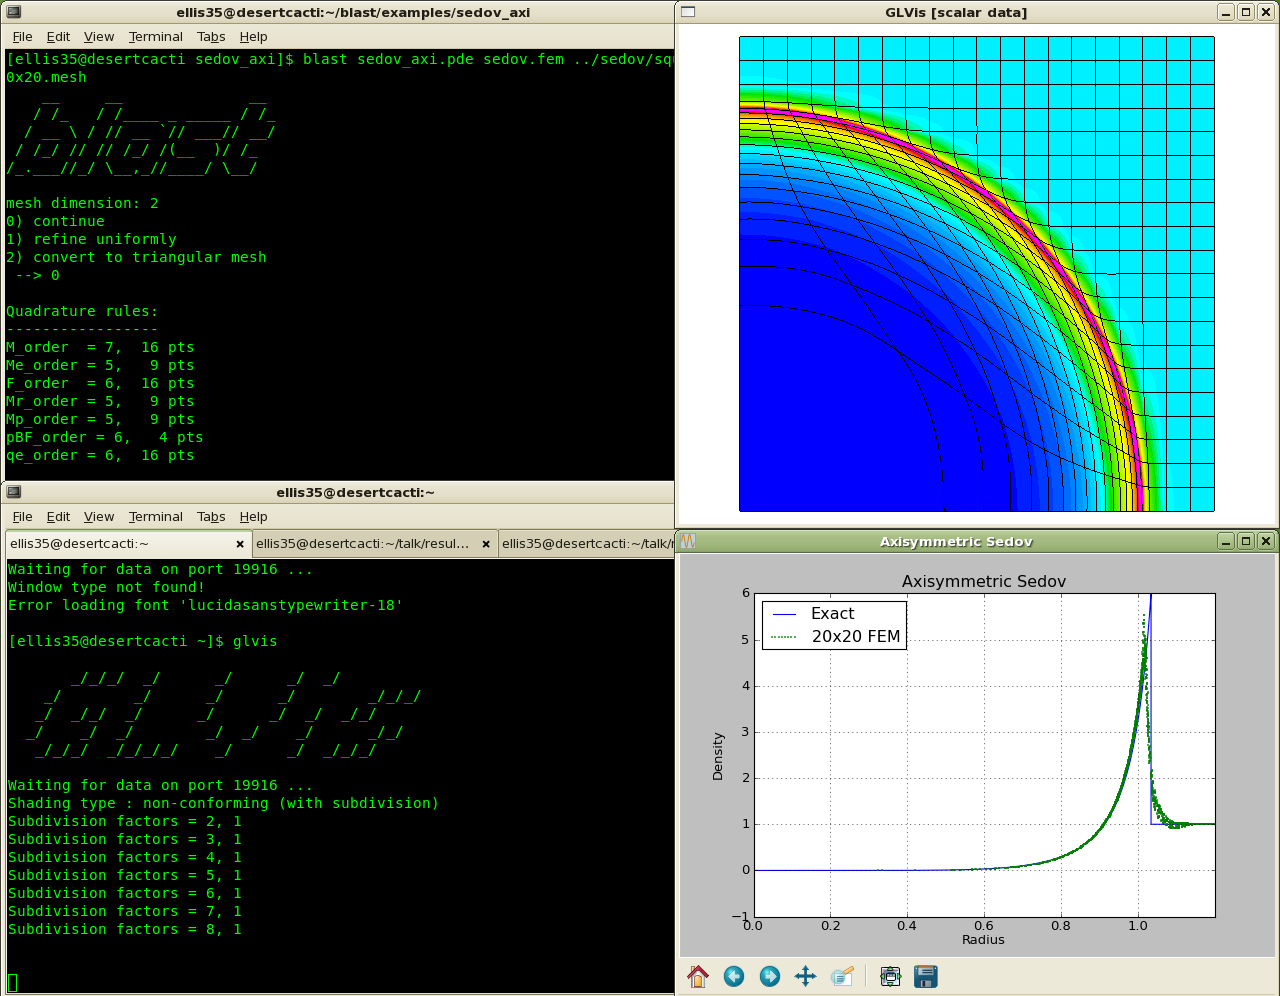
\includegraphics[width=\textwidth]{figures/Screenshot.png}
\end{column}
\end{columns}
\end{frame}

\note{
We have developed a suite of research code to implement or methods. BLAST is a
high order FEM Lagrangian hydrocode written in C++. It is built on top of MFEM,
our modular finite element library. GLVis is our FEM-aware visualization tool,
and this summer I wrote MPLVis as a Python scriptable 2D plotting tool.
}


\subsection{Numerical ICF-like Results in Cartesian Coordinates}


\begin{frame}
\frametitle{ICF-like Results in Cartesian Coordinates}
\begin{columns}
\begin{column}{0.4\textwidth}
\begin{itemize}
\item Simple 2D implosion of a cylindrical shell of ideal gas using an ICF
like pressure  drive. The interface between the high density and low
density regions is subject to both Richtmyer-Meshkov (RM) and
Rayleigh-Taylor (RT) instabilities.  \footnote[frame,1]{\tiny S. Galera, P-H. Maire, J. Breil, "A two-dimensional unstructured
cell-centered multi-material ALE scheme using VOF interface reconstruction". JCP Preprint}\\[1ex]
\item Random angular sub-divisions\\[1ex]
\item Results computed with BLAST\\[1ex]
\item Q2-Q1 spatial discretization\\[1ex]
\item RK2Avg temporal discretization ensuring exact total energy conservation
\end{itemize}
\end{column}
\begin{column}{0.6\textwidth}
\animategraphics[width=0.9\textwidth,every=2,final]{12}{
figures/simpleicf_pdrive/density}{0000}{0150}\\
\end{column}
\end{columns}
\end{frame}
\note{
I have one quick numerical problem to demonstrate why we wanted to extend this
research to axisymmetric problems. Here we have a simple 2D implosion of a
cylindrical shell of ideal gas using an ICF like pressure  drive. The interface
between the high density and low density regions is subject to both
Richtmyer-Meshkov (RM) and Rayleigh-Taylor (RT) instabilities. \\ \bigskip

Traditional SGH codes require a uniform polar mesh to achieve a symmetric
solution on this problem, but we are running on a butterfly mesh with random
angular sub-divisions. \\ \bigskip

[Play Movie] \\ \bigskip

You can see that despite the randomized mesh, we preserve symmetry. This is
because the higher order nature of our method significantly reduces mesh
imprinting on the solution.
}


\section{Axisymmetric Theory}
\note{
With those foundations laid, we can now consider extending our method to
axisymmetric problems.
}
\subsection{Introduction and Motivation}


\begin{frame}
\frametitle{Axisymmetric Hydro}
\begin{columns}[T]
\begin{column}{0.35\textwidth}
\centering
\textbf{Axisymmetric simulations are attractive computationally}
\begin{center}
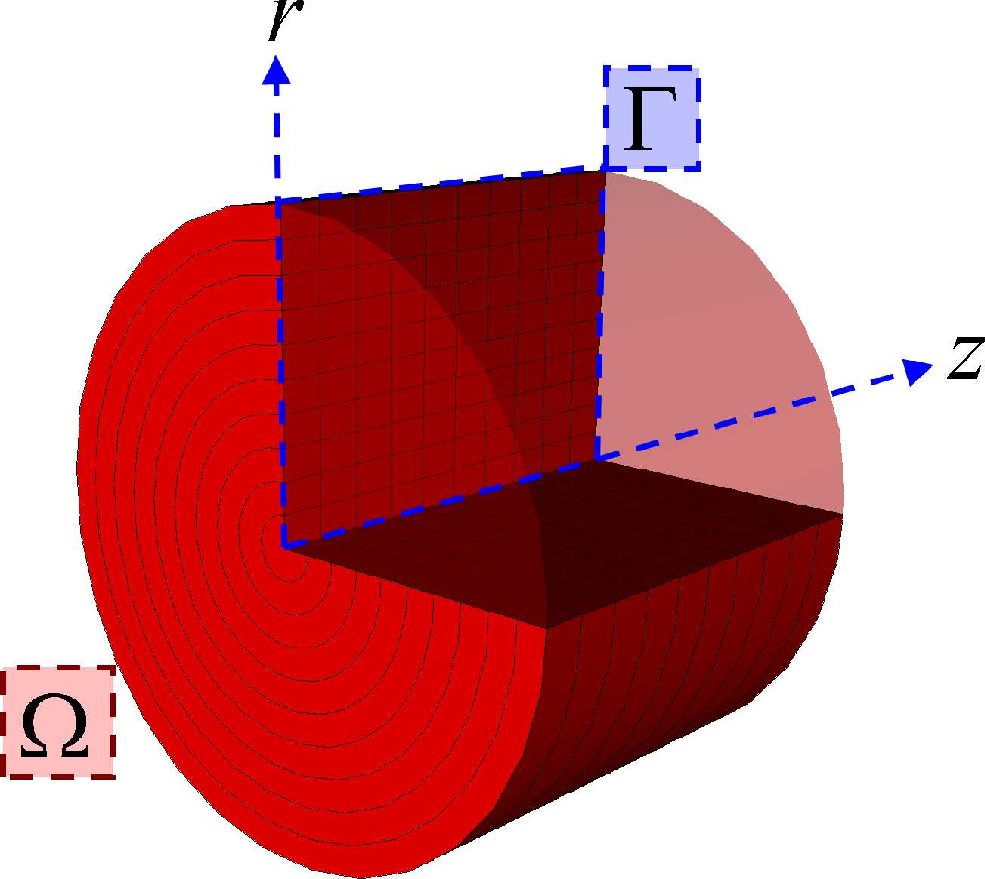
\includegraphics[width=1.0\textwidth]{figures/RZSchematic.pdf}
\end{center}
\vskip2ex
\centering
Compatibility and convergence are essential for a predictive computational
capability.
\end{column}
\begin{column}{0.6\textwidth}
\centering
\textbf{Symmetry breaking and lack of energy conservation lead to non-physical
results}
\begin{columns}[T]
\begin{column}{0.4\textwidth}
\begin{block}{\small Axisymmetric ICF Test}
\footnotesize{
ICF implosion with radial pressure drive
\vskip5pt
Initial unstructured “butterfly” mesh
\vskip5pt
\textcolor{red}{\emph{This jet is 100\% numerical and gets worse as mesh is
refined in space}}
}
\begin{center}
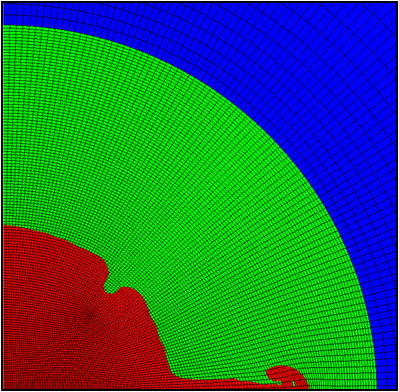
\includegraphics[height=1.0in]{figures/AxiICFOld.png}
\end{center}
\end{block}
\end{column}
\begin{column}{0.5\textwidth}
\begin{block}{\small Axisymmetric Sedov Test}
\footnotesize{
Sedov test in axi-symmetric mode
\vskip4pt
Total energy should be 1.0 for all time
\vskip4pt
Traditional PdV energy update is not conservative in r-z geometry
\vskip4pt
\textcolor{red}{\emph{Around 8.5\% artificial gain in energy. Converges under
time refinement, but not to the correct value}}
}
\begin{center}
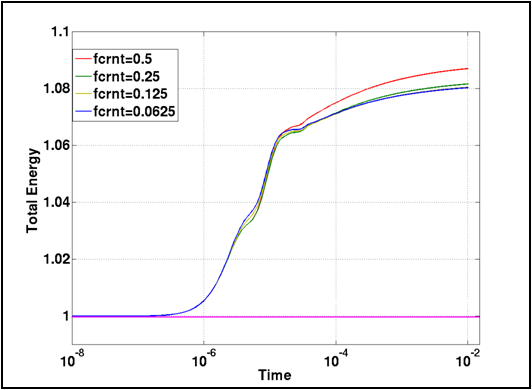
\includegraphics[height=1.0in]{figures/AxiEnergyConsOld2.png}
\end{center}
\end{block}
\end{column}
\end{columns}
\end{column}
\end{columns}
\end{frame}
\note{
Axisymmetric simulations allow us to run essentially 3D simulations in only two
dimensions. Suppose we have a body of revolution that we wish to model. The
cross-section of the problem is the same no matter which angle to the axis of
revolution that you sample it at. It would be ideal to solve our problem on just
one cut plane, $\Gamma$ and revolve that solution around the z-axis to get the
full body of revolution 3D solution. \\ \bigskip

But current SGH codes struggle with many axisymmetric simulations. Consider for
example the previous ICF-like problem run in axisymmetric mode. This would
represent the implosion of a perfectly smooth sphere, which might make a good
baseline case for NIF. But we see this jet of energy along the axis of
symmetry which is wrong and completely numerical. Symmetry is not preserved
as it should be. \\ \bigskip

Now consider the axisymmetric Sedov explosion problem. Physically we expect that
energy is not created nor destroyed, but running the Sedov problem in
cylindrical
coordinates in current SGH codes numerically creates around 8.5\% gain in
energy.
\\ \bigskip

In order to have a reliable predictive computational capability we need to get
the physics we expect and we need to converge to the correct solution under
refinement. These problems fail on both of these counts.
}


\subsection{Axisymmetric Momentum Equation}


\begin{frame}
\frametitle{Axisymmetric Momentum Equation}
\begin{minipage}[t][0.35\textheight]{\textwidth}
Rewriting the 3D momentum equation with a tensor artificial viscosity,
\[
\int_{\Omega(t)} \left(\rho\dfrac{\mathrm{d}\vec{v}}{\mathrm{d}t}\right)\cdot
\vec{w}_i
 =\int_{\Omega(t)} (p\mathbf{I}-\mu\nabla\vec{v}) :\nabla\vec{w}_i
 =-\int_{\Omega(t)} \sigma :\nabla\vec{w}_i
\]
Reducing this to the axisymmetric cut plane $\Gamma$,
\[
\visible<8->{\rlap{\color{red}\LARGE{$\searrow$}}}2\pi\int_{\Gamma(t)}r
\left(\rho\dfrac{\mathrm{d}\vec{v}}{\mathrm{d}t}\right)\cdot \vec{w}_i
=-\visible<8->{\rlap{\color{red}\LARGE{$\searrow$}}}2\pi\int_{\Gamma(t)}
r\sigma_{rz} :\nabla_{rz}\vec{w}_i
\]
\end{minipage}
\begin{overlayarea}{\textwidth}{1.0\textwidth}
% Deriving gradient of axisymmetric vector field
\only<1-7>{
% \colorbox{structure!30}{
\vskip-4ex
\begin{block}{}
% \begin{minipage}[t][0.47\textheight]{0.965\textwidth}
Applying the cylindrical gradient operator
$\nabla_{rz}f =
\frac{\partial f}{\partial r} \vec e_r +
\frac{1}{r} \frac{\partial f}{\partial \theta} \vec e_\theta +
\frac{\partial f}{\partial z} \vec e_z $

\begin{flushleft}
to the axisymmetric vector field
$\vec v = v_r(r,z) \vec e_r + v_z(r,z) \vec e_z \,,$
\end{flushleft}
\vskip-3ex
\pause
\begin{minipage}[t][0.15\textheight]{\textwidth}
\begin{columns}[b]
\begin{column}{0.6\textwidth}
\[
\nabla_{rz}\vec{v} = \frac{\partial  v_r}{\partial r}\vec e_r\otimes\vec e_r +
\frac{\partial v_z}{\partial r}\vec e_z\otimes\vec e_r +
\frac{\partial v_r}{\partial z}\vec e_r\otimes\vec e_z +
\frac{\partial v_z}{\partial z}\vec e_z\otimes\vec e_z
\]
\end{column}\hskip-2em
\begin{column}[l]{0.25\textwidth}
\begin{flushleft}{$\displaystyle
\only<4->{+}
\only<4,5>{\color{Blue}
\frac{v_r}{r}\frac{\partial\vec e_r}{\partial\theta}\otimes\vec e_{\theta}
}\only<6->{\color{Red}{
\frac{v_r}{r}\vec e_{\theta}\otimes\vec e_{\theta}}
}
$}
\end{flushleft}
\end{column}
\end{columns}
\end{minipage}
\begin{minipage}[t][0.2\textheight]{\textwidth}
\only<2,3>{
\[
+ \frac{1}{r}\left(\visible<3>{\rlap{\color{red}\LARGE{$\searrow$}}}
\frac{\partial v_r}{\partial \theta}\vec e_r\otimes\vec e_{\theta} +
v_r\frac{\partial \vec e_r}{\partial \theta}\otimes\vec e_{\theta} +
\visible<3>{\rlap{\color{red}\LARGE{$\searrow$}}}
\frac{\partial v_z}{\partial \theta}\vec e_z\otimes\vec e_{\theta} +
\visible<3>{\rlap{\color{red}\LARGE{$\searrow$}}}
\frac{\partial \vec e_z}{\partial \theta}\vec v_z\otimes\vec e_\theta
\right)
\]
}
\only<5>{
Recall
\[
\vec e_r = (\cos\theta,\sin\theta,0)\,,\quad
\vec e_{\theta} = (-\sin\theta,\cos\theta,0)\,,\quad
\vec e_z = (0,0,1)
\]
}
\only<7->{
Thus, the axisymmetric velocity gradient is
\[
\nabla_{rz} \vec v =
\begin{pmatrix}
\frac{\partial v_z }{\partial z} & \frac{\partial v_z }{\partial r} & 0 \\
\frac{\partial v_r }{\partial z} & \frac{\partial v_r }{\partial r} & 0 \\
0 & 0 & \frac{v_r}{r}
\end{pmatrix}_{z-r-\theta}
=
\begin{pmatrix}
\nabla_{2d} \vec v & 0 \\
 0 & \frac{v_r}{r}
\end{pmatrix}
\]
}
\end{minipage}
% \end{minipage}
% }
\end{block}
}
% Finishing momentum equation
\only<8->{\begin{minipage}[t][0.4\textheight]{\textwidth}
\only<9->{
\vskip-4ex
\begin{block}{}
For $\sigma = -p\mathbf{I}+\mu\nabla\vec{v}$, the axisymmetric stress
tensor is
$$
\sigma_{rz} = \begin{pmatrix}
-p\mathbf{I}+\mu\nabla_{2d} \vec{v} & 0 \\
 0 & -p+\mu\frac{v_r}{r}
\end{pmatrix}
$$
\end{block}
The axisymmetric momentum equation becomes
\[
\int_{\Gamma(t)}\color<12>{Red}{r}\color{Black}
\left(\rho\dfrac{\mathrm{d}\vec{v}}{\mathrm{d}t}\right)\cdot \vec{w}_i
=-\int_{\Gamma(t)} r
\begin{pmatrix}
\sigma_{2d} & 0 \\
 0 & -p+\mu\frac{v_r}{r}
\end{pmatrix}
 :
\begin{pmatrix}
\nabla_{2d} \vec w_i & 0 \\
 0 & \frac{w_r}{r}
\end{pmatrix}
\]
\uncover<10-12>{
\alt<10>{
\[
=-\int_{\Gamma(t)}r\left[\left(\sigma_{2d}:\nabla_{2d}\vec w_i\right)
 - p\frac{w_r}{r} + \mu\frac{v_r w_r}{r^2} \right]
\]}
{
\[
=-\int_{\Gamma(t)}\color<12>{Red}{r}\color{Black}{\left(\sigma_{2d}:\nabla_{2d}
\vec w_i\right)}
 \color<12>{Red}{- p w_r + \mu\frac{v_r w_r}{r}}
\]}
}
}
\end{minipage}}
\end{overlayarea}
\end{frame}
\note{
Starting with the weak form of our full 3D momentum equation. We can reduce this
to the axisymmetric cut plane: $\Gamma$. This gives us a factor of $2\pi r$ in
our integrals, and we now have to deal with the axisymmetric stress tensor and
gradient term. Let's first evaluate this gradient term.\\ \bigskip

Applying the chain rule to the cylindrical gradient operator acting on the
axisymmetric vector field $\vec v$,
(page down) \\
we get the following long expression. Noting that our vector field is
axisymmetric, several of these terms become zero.
(page down)\\
and only one of these last four terms remains.
(page down)\\
Recalling the coordinate vectors in cylindrical coordinates,
$\frac{\partial \vec e_r}{\partial \theta}$ becomes $\vec e_\theta$.
(page down)\\
And our axisymmetric velocity gradient becomes the following 3x3 tensor. The
upper left block looks exactly like the 2 dimensional gradient operator. So in
essence, we just have our 2D gradient operator with an additional term in the
$\theta$ diagonal spot.
(page down)\\ \bigskip
Returning to our momentum equation and canceling the $2\pi$ terms.
(page down)\\
We can define our axisymmetric stress tensor. Which looks just like our 2D
stress
tensor with an extra term in the $\theta$ diagonal spot. When we put everything
together in the momentum equation, we get the following.
(page down)\\
And when we contract these two matrices together, we get this expression.
(page down)\\
Multiplying out the $r$ term (page down)\\
And we get the following momentum equation where all of the red terms are the
additional terms that we need to add to our 2D code to model axisymmetric
problems.
}


\subsection{Semi-discrete Axisymmetric Method}


\begin{frame}
\frametitle{Semi-discrete Axisymmetric Method}

Axisymmetric mass matrices \hskip2em
$\displaystyle
\mathbf{M}^{rz}_v=\int_{\Gamma(t)}r \rho \mathbf{w} \mathbf{w}^T \qquad
\mathbf{M}^{rz}_e=\int_{\Gamma(t)}r \rho \boldsymbol{\phi} \boldsymbol{\phi}^T
$ \\[2ex]
Axisymmetric generalized corner force matrix
\[
(\mathbf{F}^{rz})_{ij}= \int_{\Gamma(t)} r \left(\sigma_{rz}:\nabla_{rz}
\vec{w}_i\right)\phi_j
\]
We can rewrite our equations:
\begin{columns}
\begin{column}{0.35\textwidth}
\begin{block}{\centering Conservation of Momentum}
\[
\mathbf{M}^{rz}_v\frac{\mathrm{d}\mathbf{v}}{\mathrm{d}t}=- \mathbf{F}^{rz}\cdot
\mathbf{1}
\]
\end{block}
\end{column}
\begin{column}{0.35\textwidth}
\begin{block}{\centering Conservation of Energy}
\[
\mathbf{M}^{rz}_e\frac{\mathrm{d}\mathbf{e}}{\mathrm{d}t}=(\mathbf{F}^{rz}
)^T\cdot \mathbf{v}
\]
\end{block}
\end{column}
\end{columns}
\vskip2ex
The axisymmetric strong mass conservation principle reads
\colorbox{cyan!20}{
$
r(t) \rho(t)|\mathbf{J}(t)|= r(t_0) \rho(t_0)|\mathbf{J}(t_0)|
$}
which implies
\[
\frac{\mathrm{d}\mathbf{M}^{rz}_v}{\mathrm{d}t}=0, \qquad
\frac{\mathrm{d}\mathbf{M}^{rz}_e}{\mathrm{d}t}=0
\]
and the exact axisymmetric semi-discrete energy conservation:
\[
\frac{\mathrm{d}E^{rz}}{\mathrm{d}t}=
\frac{\mathrm{d}}{\mathrm{d}t}
\left( \int_{\Omega(t)} \rho \frac{|\vec{v}|^2}{2} + \rho e \right)
=
\frac{\mathrm{d}}{\mathrm{d}t}
\left( 2 \pi \int_{\Gamma(t)} r \rho \frac{|\vec{v}|^2}{2} + r \rho e \right)
= 0.
\]
\end{frame}
\note{
With this, we can define our semi-discrete axisymmetric method. Our mass
matrices
are defined as before with and additional $r$ weighting. \\ \bigskip

If we add an $r$ weighting and the modified stress tensor and axisymmetric
velocity gradient term, we get our axisymmetric generalized corner forces.\\
\bigskip

With these basic modifications, we can rewrite our conservation equations just
as before. \\ \bigskip

Our strong mass conservation now includes a radial weighting term, but still
implies constant mass matrices. \\ \bigskip

Furthermore, we still get exact semi-discrete total energy conservation.
}


\section{Axisymmetric Numerical Results}
\note{
So I actually implemented this in BLAST. We can take any 2D problem description
file and add a flag to run it axisymmetric, and BLAST will use these modified
terms to solve the full axisymmetric problem. \\ \bigskip

So now we have a few numerical results to test our method on several important
aspects of axisymmetric problems. We would like to see symmetry preservation
on problems that should preserve symmetry, exact total energy conservation, and
robustness to problems with complicated flow physics.
}
\subsection{Axisymmetric Coggeshall Convergence}


\begin{frame}
\frametitle{Axisymmetric Coggeshall Q2-Q1 Convergence}
\begin{columns}
\begin{column}{0.4\textwidth}
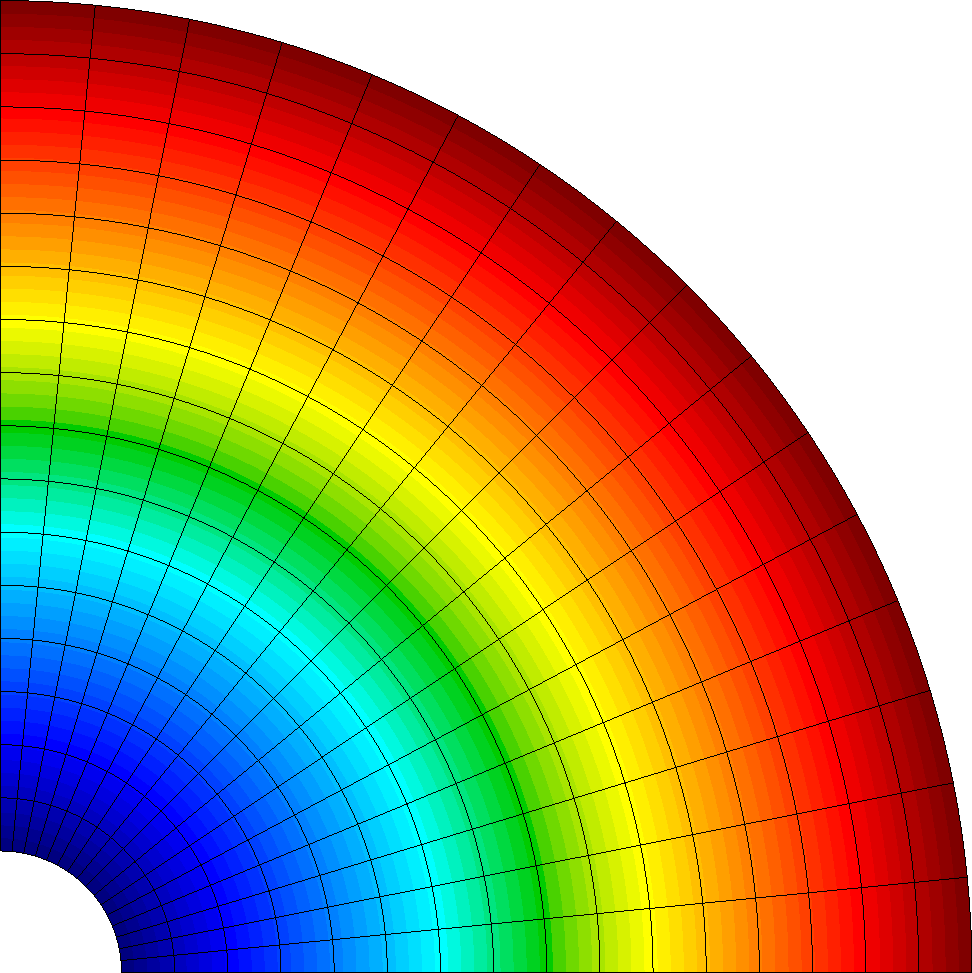
\includegraphics[width=0.9\textwidth]{figures/CoggMesh_Q2Q1.png}
\begin{itemize}
\item Coggeshall\footnote[1]{\tiny S. Coggeshall, "Analytic solutions of
hydrodynamics equations," Physics of Fluids, 1991} self-similar adiabatic
compression problem \# 1
\item Curved structured annular mesh
\item Q2-Q1 Finite Elements
\item RK2Avg time step
\end{itemize}
\bigskip
\end{column}
\begin{column}{0.45\textwidth}
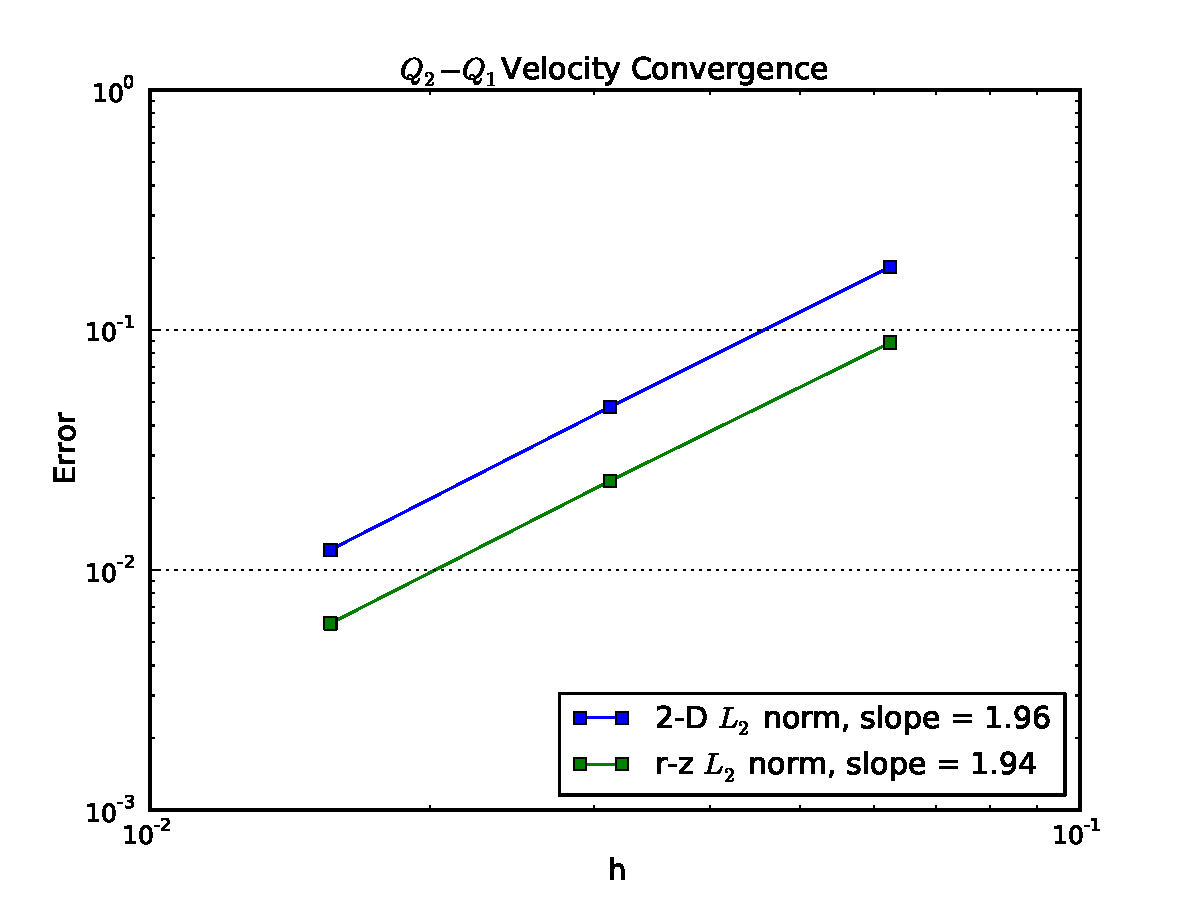
\includegraphics[width=1\textwidth]{figures/CoggErrorQ2Q1_V.pdf}
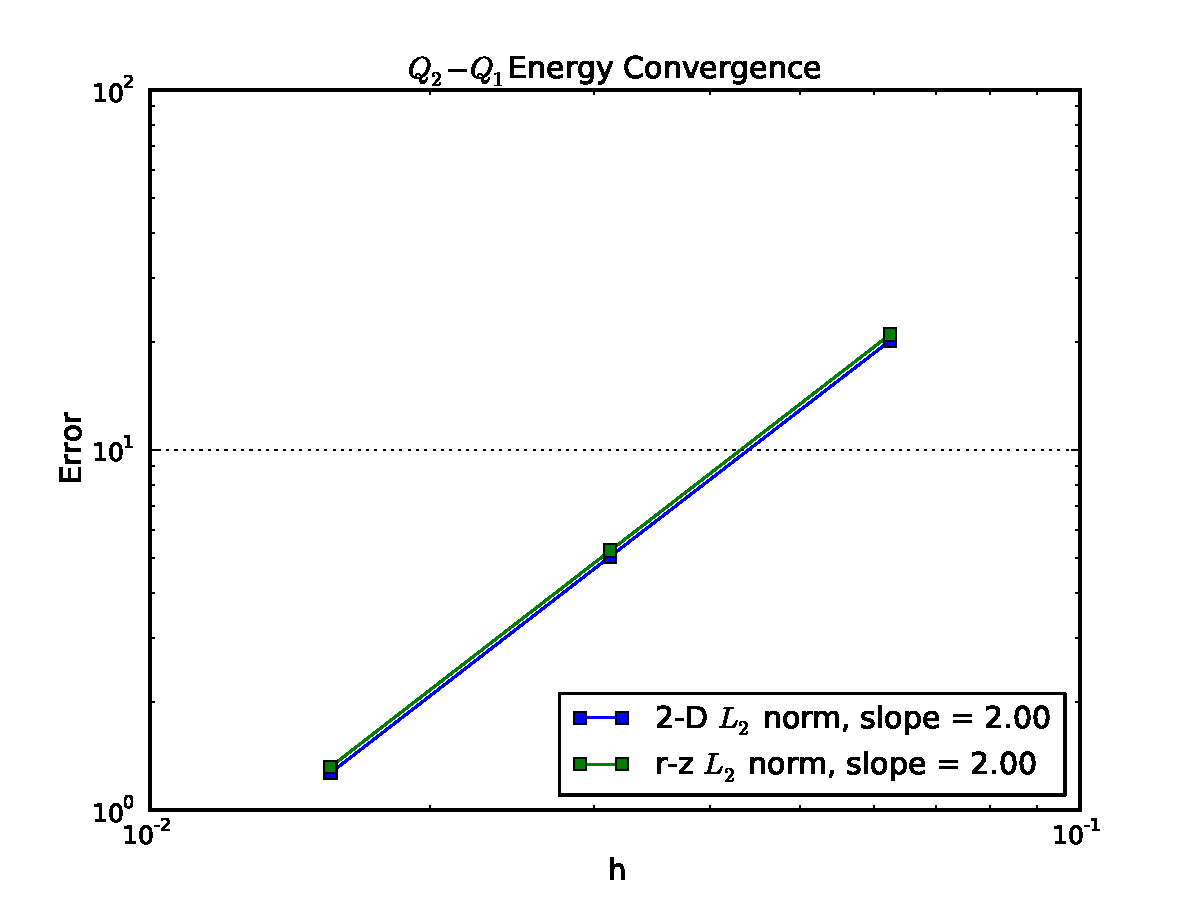
\includegraphics[width=1\textwidth]{figures/CoggErrorQ2Q1_E.pdf}
\end{column}
\end{columns}
\end{frame}
\note{
Here we have the Coggeshall self-similar adiabatic compression problem \# 1.
Ideally we should see the original mesh scale down as the problem progresses,
which is exactly what we observe. This is also a smooth problem without shocks,
so we can test the convergence of our method. \\ \bigskip

We used the bi-quadratic velocity, bi-linear energy Q2-Q1 element in this test
with a modified energy conserving Runge-Kutta time step on a structured annular
mesh. We were easily able to achieve second order convergence to the exact
solution.
}


\begin{frame}
\frametitle{Axisymmetric Coggeshall Q3-Q2 Convergence}
\begin{columns}
\begin{column}{0.4\textwidth}
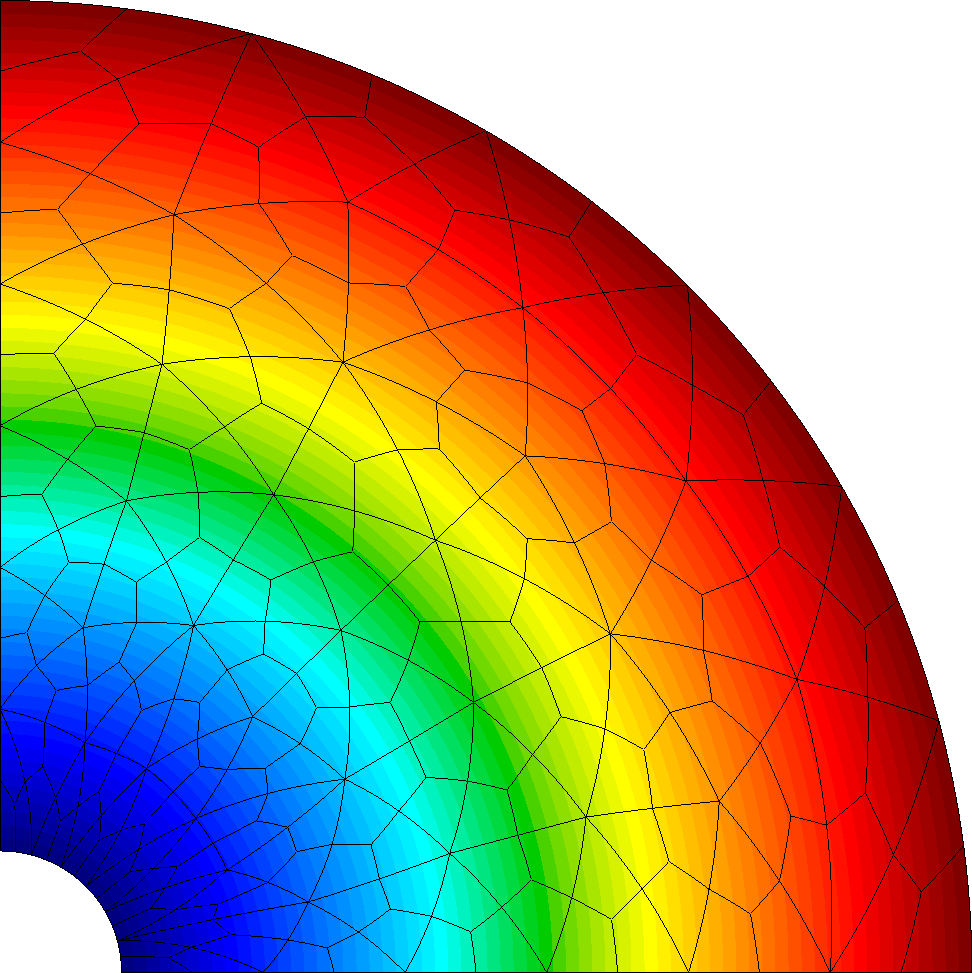
\includegraphics[width=0.9\textwidth]{figures/CoggMesh_Q3Q2.png}
\begin{itemize}
\item Coggeshall\footnote[1]{\tiny S. Coggeshall, "Analytic solutions of
hydrodynamics equations," Physics of Fluids, 1991} self-similar adiabatic
compression problem \# 1
\item Curved unstructured annular mesh
\item Q3-Q2 Finite Elements
\item RK4 time step
\end{itemize}
\bigskip
\end{column}
\begin{column}{0.45\textwidth}
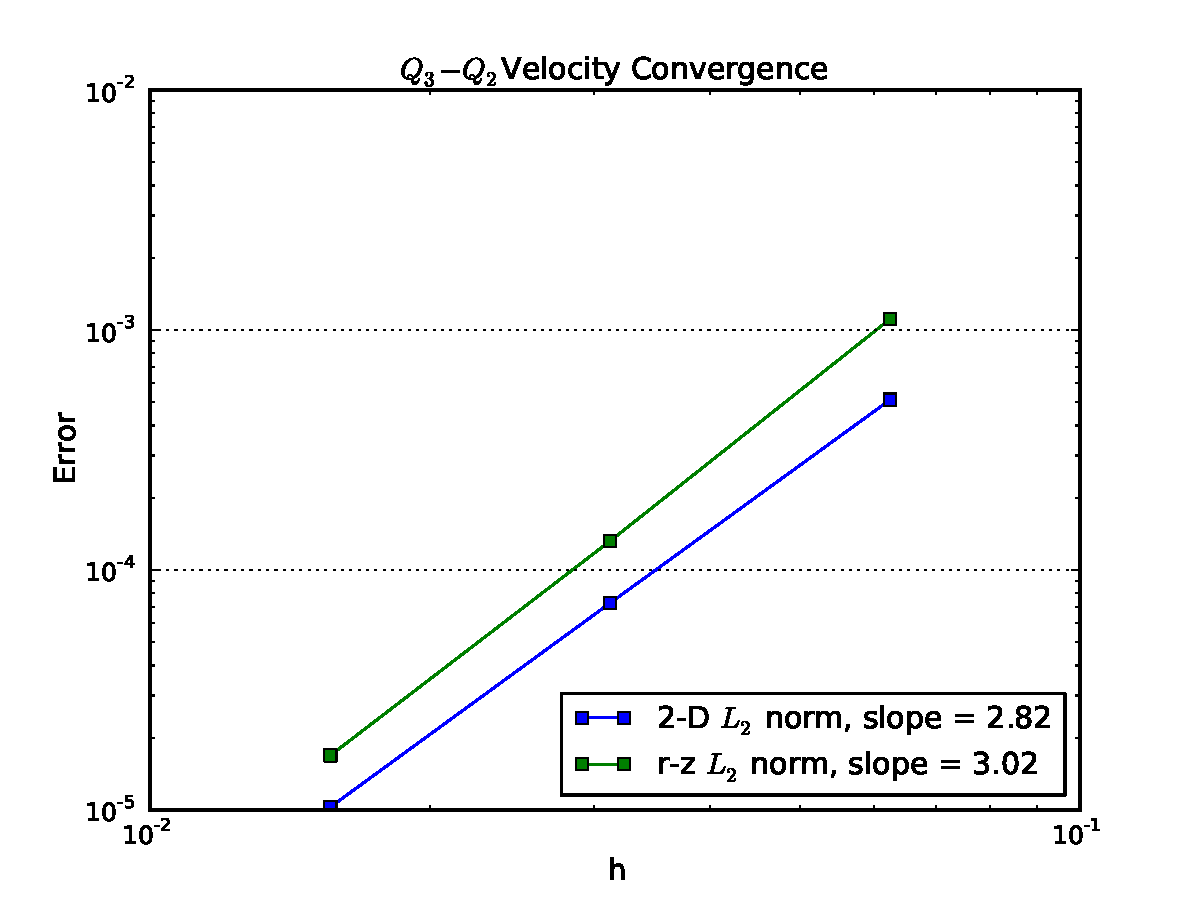
\includegraphics[width=1\textwidth]{figures/CoggErrorQ3Q2_V.pdf}
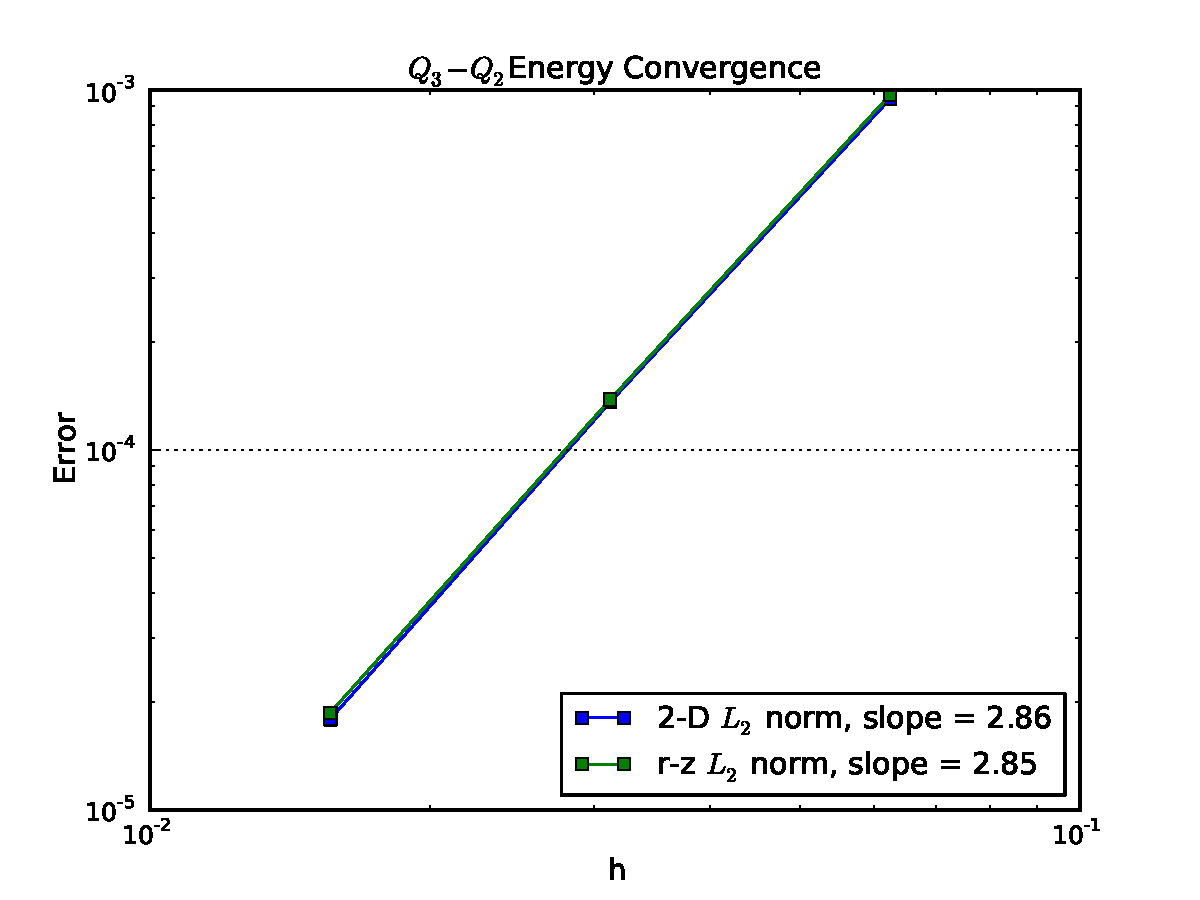
\includegraphics[width=1\textwidth]{figures/CoggErrorQ3Q2_E.pdf}
\end{column}
\end{columns}
\end{frame}
\note{
But our high order convergence is not limited to structured meshes or just Q2-Q1
elements (although that that is our workhorse, and all of our following results
will be with that element). We were able to achieve third order convergence with
the Q3-Q2 element on this unstructured mesh with a Runge-Kutta 4 time step.
\\ \bigskip

(pause)
}


\subsection{Axisymmetric Sedov Explosion}


\begin{frame}
\frametitle{Axisymmetric Sedov Explosion}
\begin{columns}
\begin{column}{0.5\textwidth}
\begin{center}
40x40 Lagrangian SGH - Density
\animategraphics[width=1\textwidth,every=2,final]{12}{
figures/SedovSGH_40x40/sedovaxi_40x40_sgh}{0000}{0100}
\begin{itemize}
\item Symmetry is not preserved
\item Mesh distorted near the origin
\end{itemize}
\end{center}
\end{column}
\begin{column}{0.5\textwidth}
\begin{center}
20x20 Lagrangian FEM - Density
\animategraphics[width=1\textwidth,every=2,final]{12}{
figures/SedovFEM_20x20/sedovaxi_20x20_fem}{0000}{0100}
\begin{itemize}
\item Symmetry is preserved
\item Curvilinear zones match physics
\end{itemize}
\end{center}
\end{column}
\end{columns}
\end{frame}
\note{
Now let's take a look at the axisymmetric Sedov problem. This is the problem
that
we looked at earlier which motivated the use of higher order elements. If we
take an initially cartesian mesh and introduce a large amount of energy into the
original zone, a blast wave will travel radially away from the origin. In
cylindrical coordinates this becomes a full spherical explosion. \\ \bigskip

Now let's see how traditional SGH works on this problem. \\ \medskip
(play movie)\\ \bigskip

We can see that symmetry is not preserved and that the original zone is pulled
along the axis of symmetry, a common problem in axisymmetric SGH simulations.
\\ \bigskip

Let's see how our method does using our default Q2-Q1 finite elements. \\
\medskip
(play movie)\\ \bigskip

We conserve symmetry much better and the curved zones more accurately match the
physics of the problem.
}


\begin{frame}
\frametitle{Axisymmetric Sedov - Scatter Plots}
\begin{columns}[T]
\begin{column}{0.5\textwidth}
\begin{center}
\small
Coarse Mesh Scatter Plot of Density vs Radius
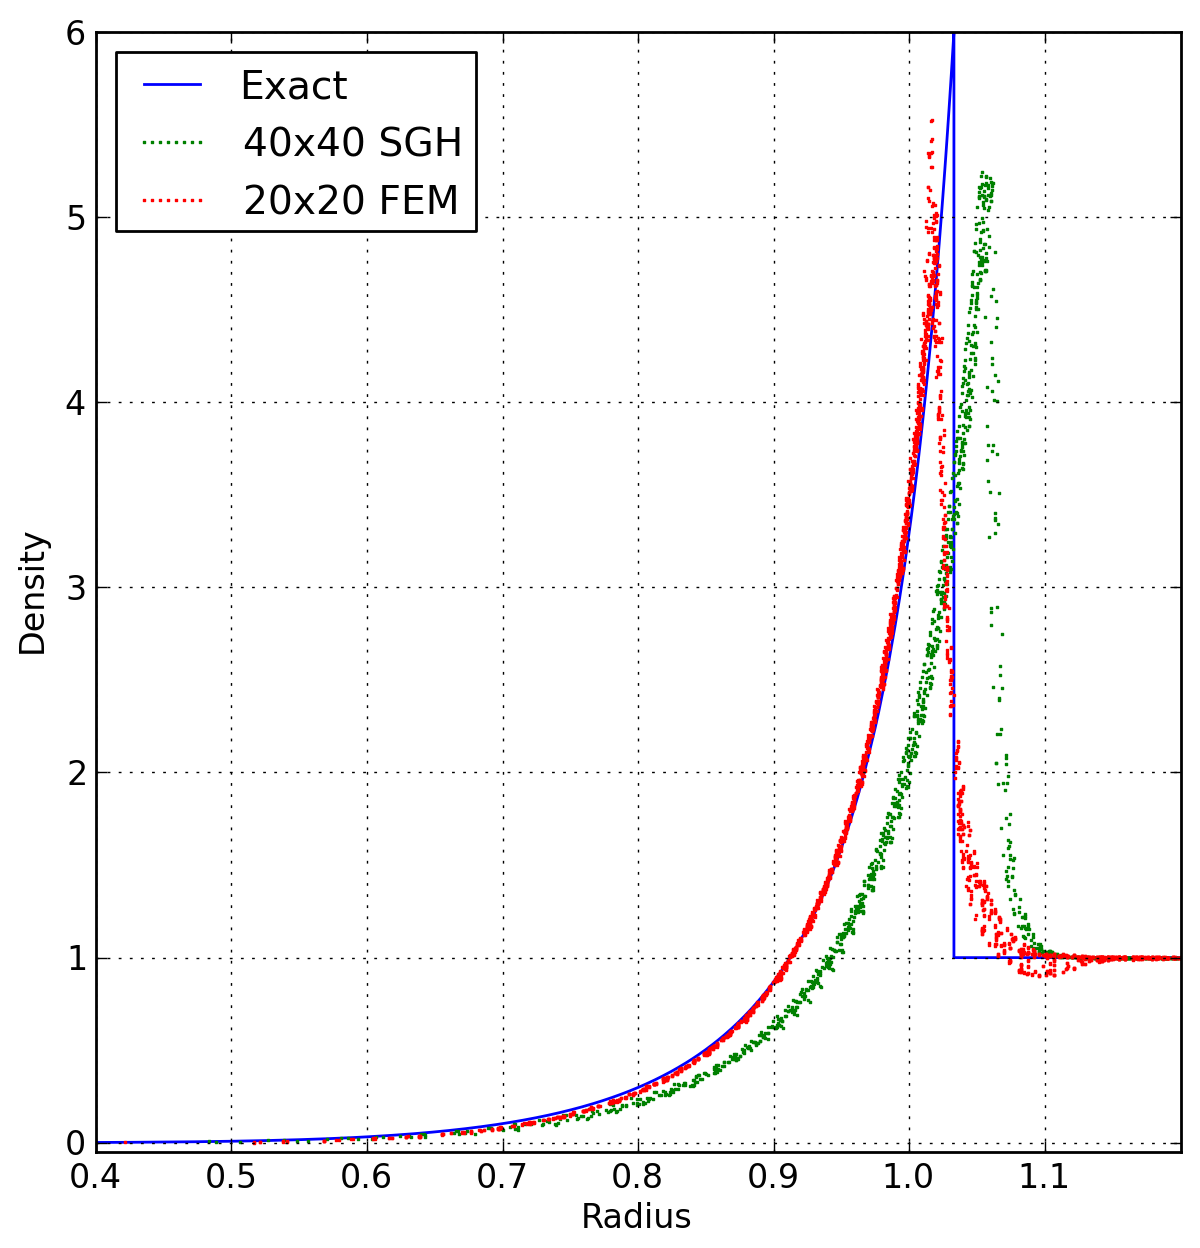
\includegraphics[width=1\textwidth]{figures/CodeComparison_SedovLow.png}
\vskip-2ex
\begin{itemize}
\item SGH shock is too fast
\item FEM is good with only 20x20 zones
\end{itemize}
\end{center}
\end{column}
\begin{column}{0.5\textwidth}
\begin{center}
\small
Fine Mesh Scatter Plot of Density vs Radius
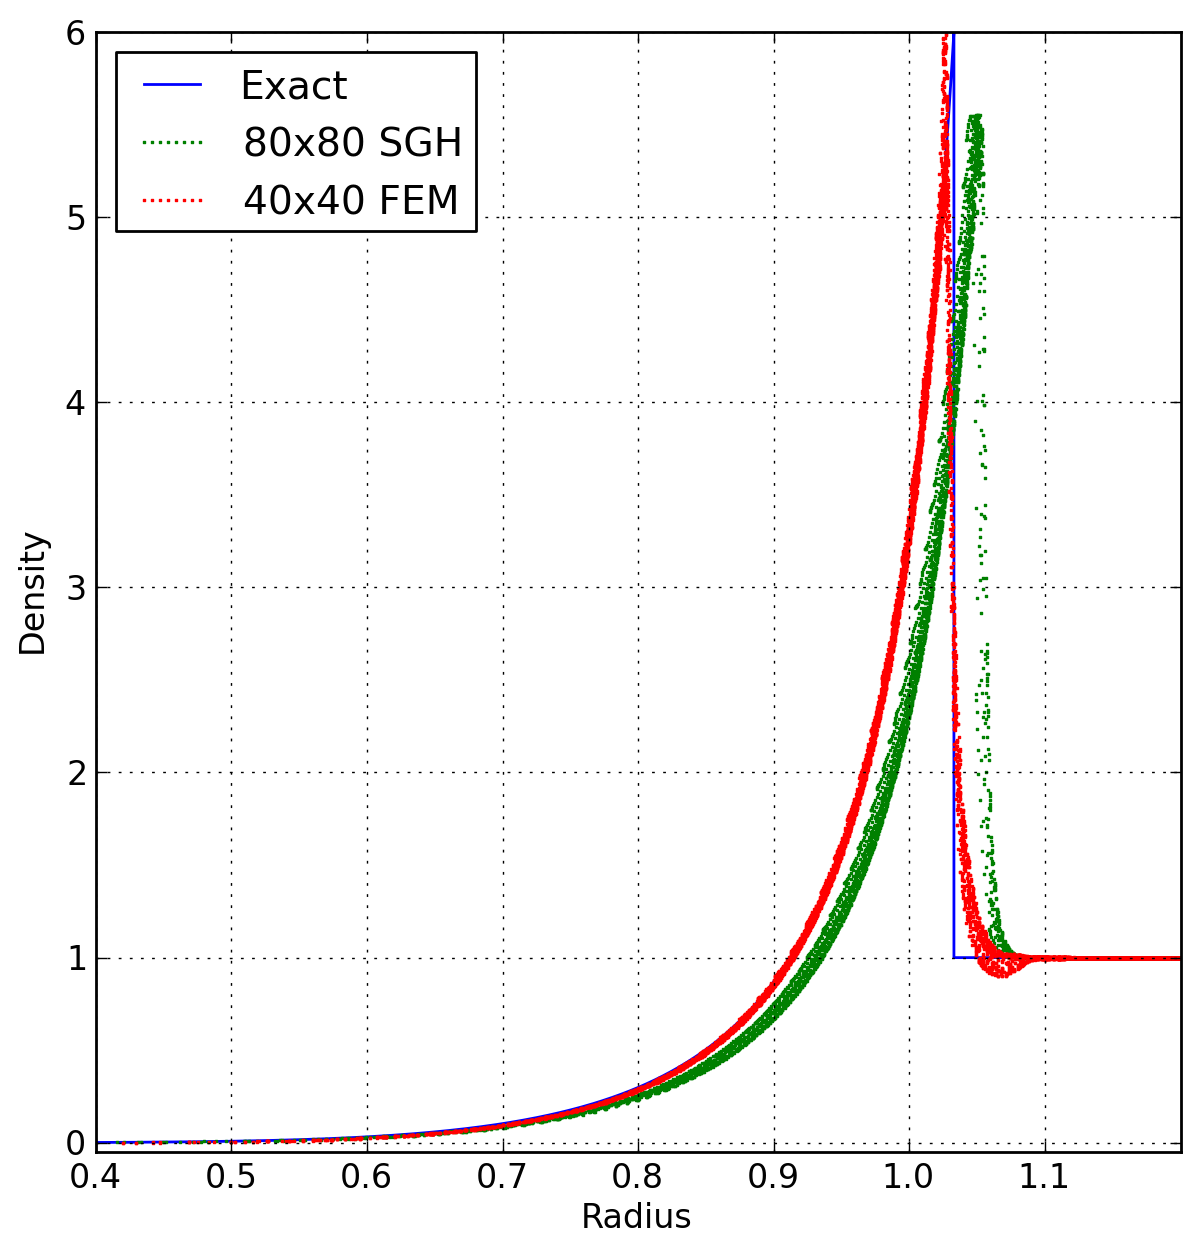
\includegraphics[width=1\textwidth]{figures/CodeComparison_SedovHigh.png}
\vskip-2ex
\begin{itemize}
\item SGH does not improve under refinement
\item FEM matches exact solution very closely
\end{itemize}
\end{center}
\end{column}
\end{columns}
\end{frame}
\note{
Now let's see how those results look in a scatter plot. In order to be fair, we
need to double the resolution of the SGH simulations to have an equal DOF count.
\\ \bigskip

The first thing we notice is that the SGH shock traveled too far in relation to
the exact solution. And this doesn't get much better under refinement. The FEM
solution on the other hand matches pretty closely with only 20x20 zones and
is almost indistinguishable from the exact solution at 40x40.
}


\begin{frame}
\frametitle{Axisymmetric Sedov - Energy Conservation}
\begin{columns}[T]
\begin{column}{0.5\textwidth}
\begin{center}
\small
Comparison of Energy Conservation
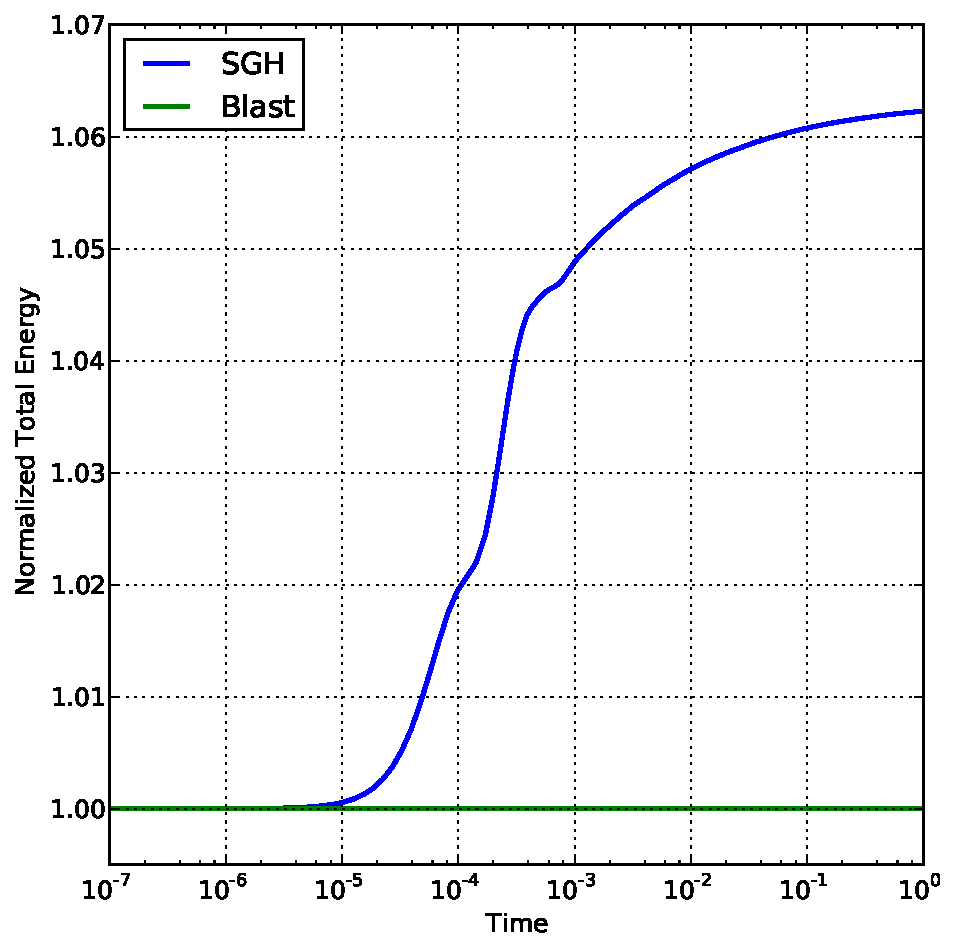
\includegraphics[width=1\textwidth]{figures/EnergyCons_Sedov.pdf}
\vskip-2ex
\begin{itemize}
\item SGH gains 6\% energy
\item BLAST conserves energy to machine precision
\end{itemize}
\end{center}
\end{column}
\begin{column}{0.5\textwidth}
\begin{center}
\small
BLAST Energy Transfer
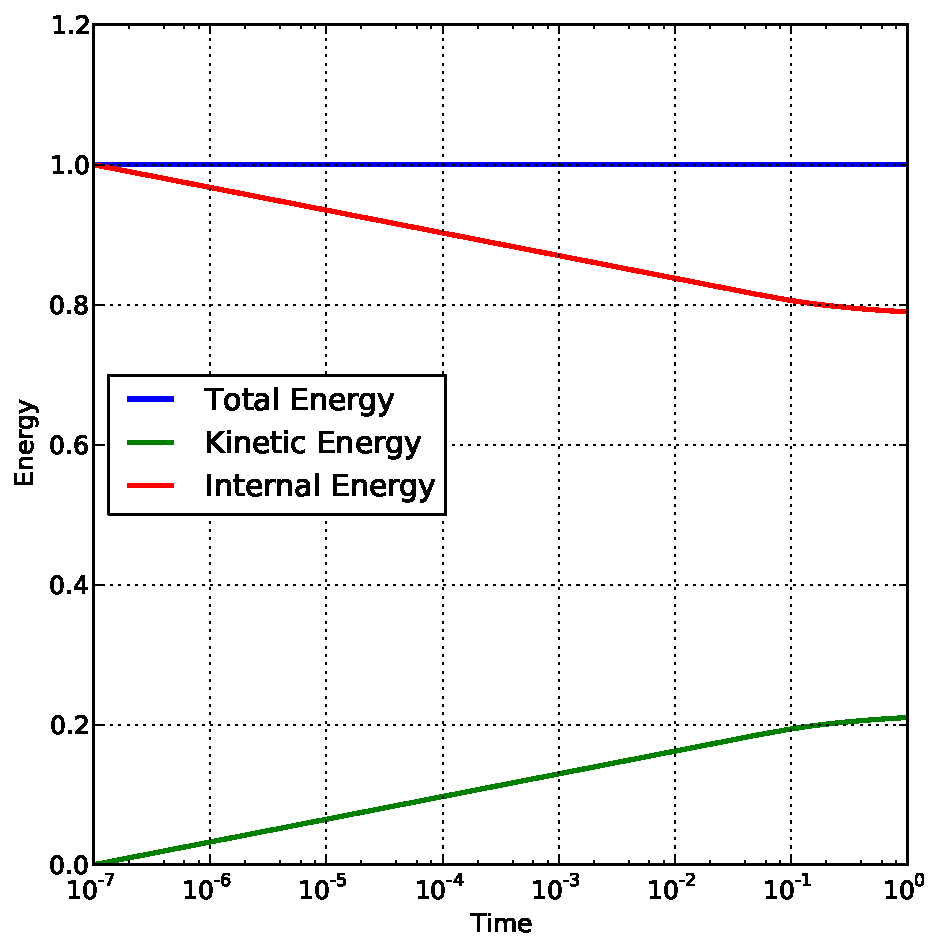
\includegraphics[width=1\textwidth]{figures/EnergyConv_Sedov.pdf}
\vskip-2ex
\begin{itemize}
\item BLAST converts IE to KE without loss
\end{itemize}
\end{center}
\end{column}
\end{columns}
\end{frame}
\note{
Let's see why the SGH shock traveled too fast. According to this energy
conservation plot, SGH gained about 6 \% energy during the simulation. It is
natural that adding energy to an explosion would propel the shock further.
\\ \bigskip

BLAST on the other hand converts from IE to KE without loss.
}


\subsection{Axisymmetric Noh Implosion}


\begin{frame}
\frametitle{Axisymmetric Noh Implosion}
\begin{columns}[T]
\begin{column}{0.5\textwidth}
\begin{center}
\alt<1>{
32x32 Lagrangian SGH
\animategraphics[width=1\textwidth,every=2,final]{12}{
figures/NohSGHLag_32x32/nohaxi_sgh_lag_32by32}{0000}{0100}
\begin{itemize}
\item Symmetry is not preserved
\item Mesh distorted near the origin
\end{itemize}
}{
64x64 Arbitrary Lagrangian Eulerian SGH
\animategraphics[width=1\textwidth,every=2,final]{12}{
figures/NohSGH_ALE_64x64/nohaxi_sgh_ale_64by64}{0000}{0100}
\begin{itemize}
\item ALE fixes mesh
\item Energy jets from wall heating
\end{itemize}
}
\end{center}
\end{column}
\begin{column}{0.5\textwidth}
\begin{center}
\only<1>{
32x32 Lagrangian FEM
\animategraphics[width=1\textwidth,every=2,final]{12}{
figures/NohFEM_32x32/nohaxi_fem_lag_32by32}{0000}{0100}
}
\only<2>{
32x32 Lagrangian FEM
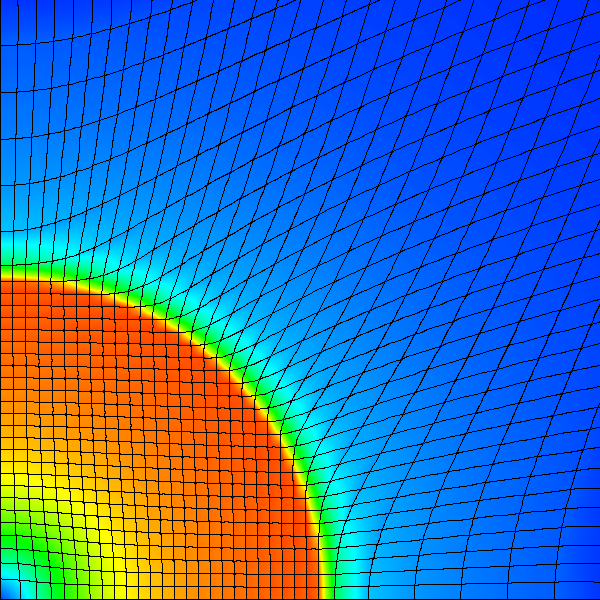
\includegraphics[width=1\textwidth]{
figures/NohFEM_32x32/nohaxi_fem_lag_32by320100.png}
}
\vskip-3.2ex
\begin{itemize}
\item Symmetry is preserved
\item Wall heating is typical for Lagrangian methods
\end{itemize}
\end{center}
\end{column}
\end{columns}
\end{frame}
\note{
The Noh implosion is almost the opposite kind of problem in that it converts KE
to IE. We initialize the velocity of every particle to be radially inward. As
the fluid collides at the origin, a shock wave propagates radially outward at
a speed of 1/3. Lagrangian simulations suffer from numerical wall heating at the
origin which artificially increases the density of the zones close to the
origin. Let's see how SGH does on this problem.\\
(play movie)\\ \bigskip

We can see that symmetry is not preserved and the mesh gets very distorted near
the origin. Now let's see how BLAST does on the same mesh.\\
(play movie)\\ \bigskip

We can see that symmetry is preserved with our FEM formulation. But to be fair
we need to compare SGH with a refined mesh. We tried this, but the mesh
distortion near the origin causes the higher resolution simulation to crash. The
only way that we could get the solution to proceed was to turn on ALE mesh
relaxation. So let's see how SGH with ALE does.\\
(play movie)\\ \bigskip

ALE definitely fixes the mesh, but symmetry is still not preserved as can be
seen by the presence of energy jets along the axis.
}


\begin{frame}
\frametitle{Axisymmetric Noh - Symmetry Preservation}
\begin{columns}[T]
\begin{column}{0.5\textwidth}
\begin{center}
Code Comparison
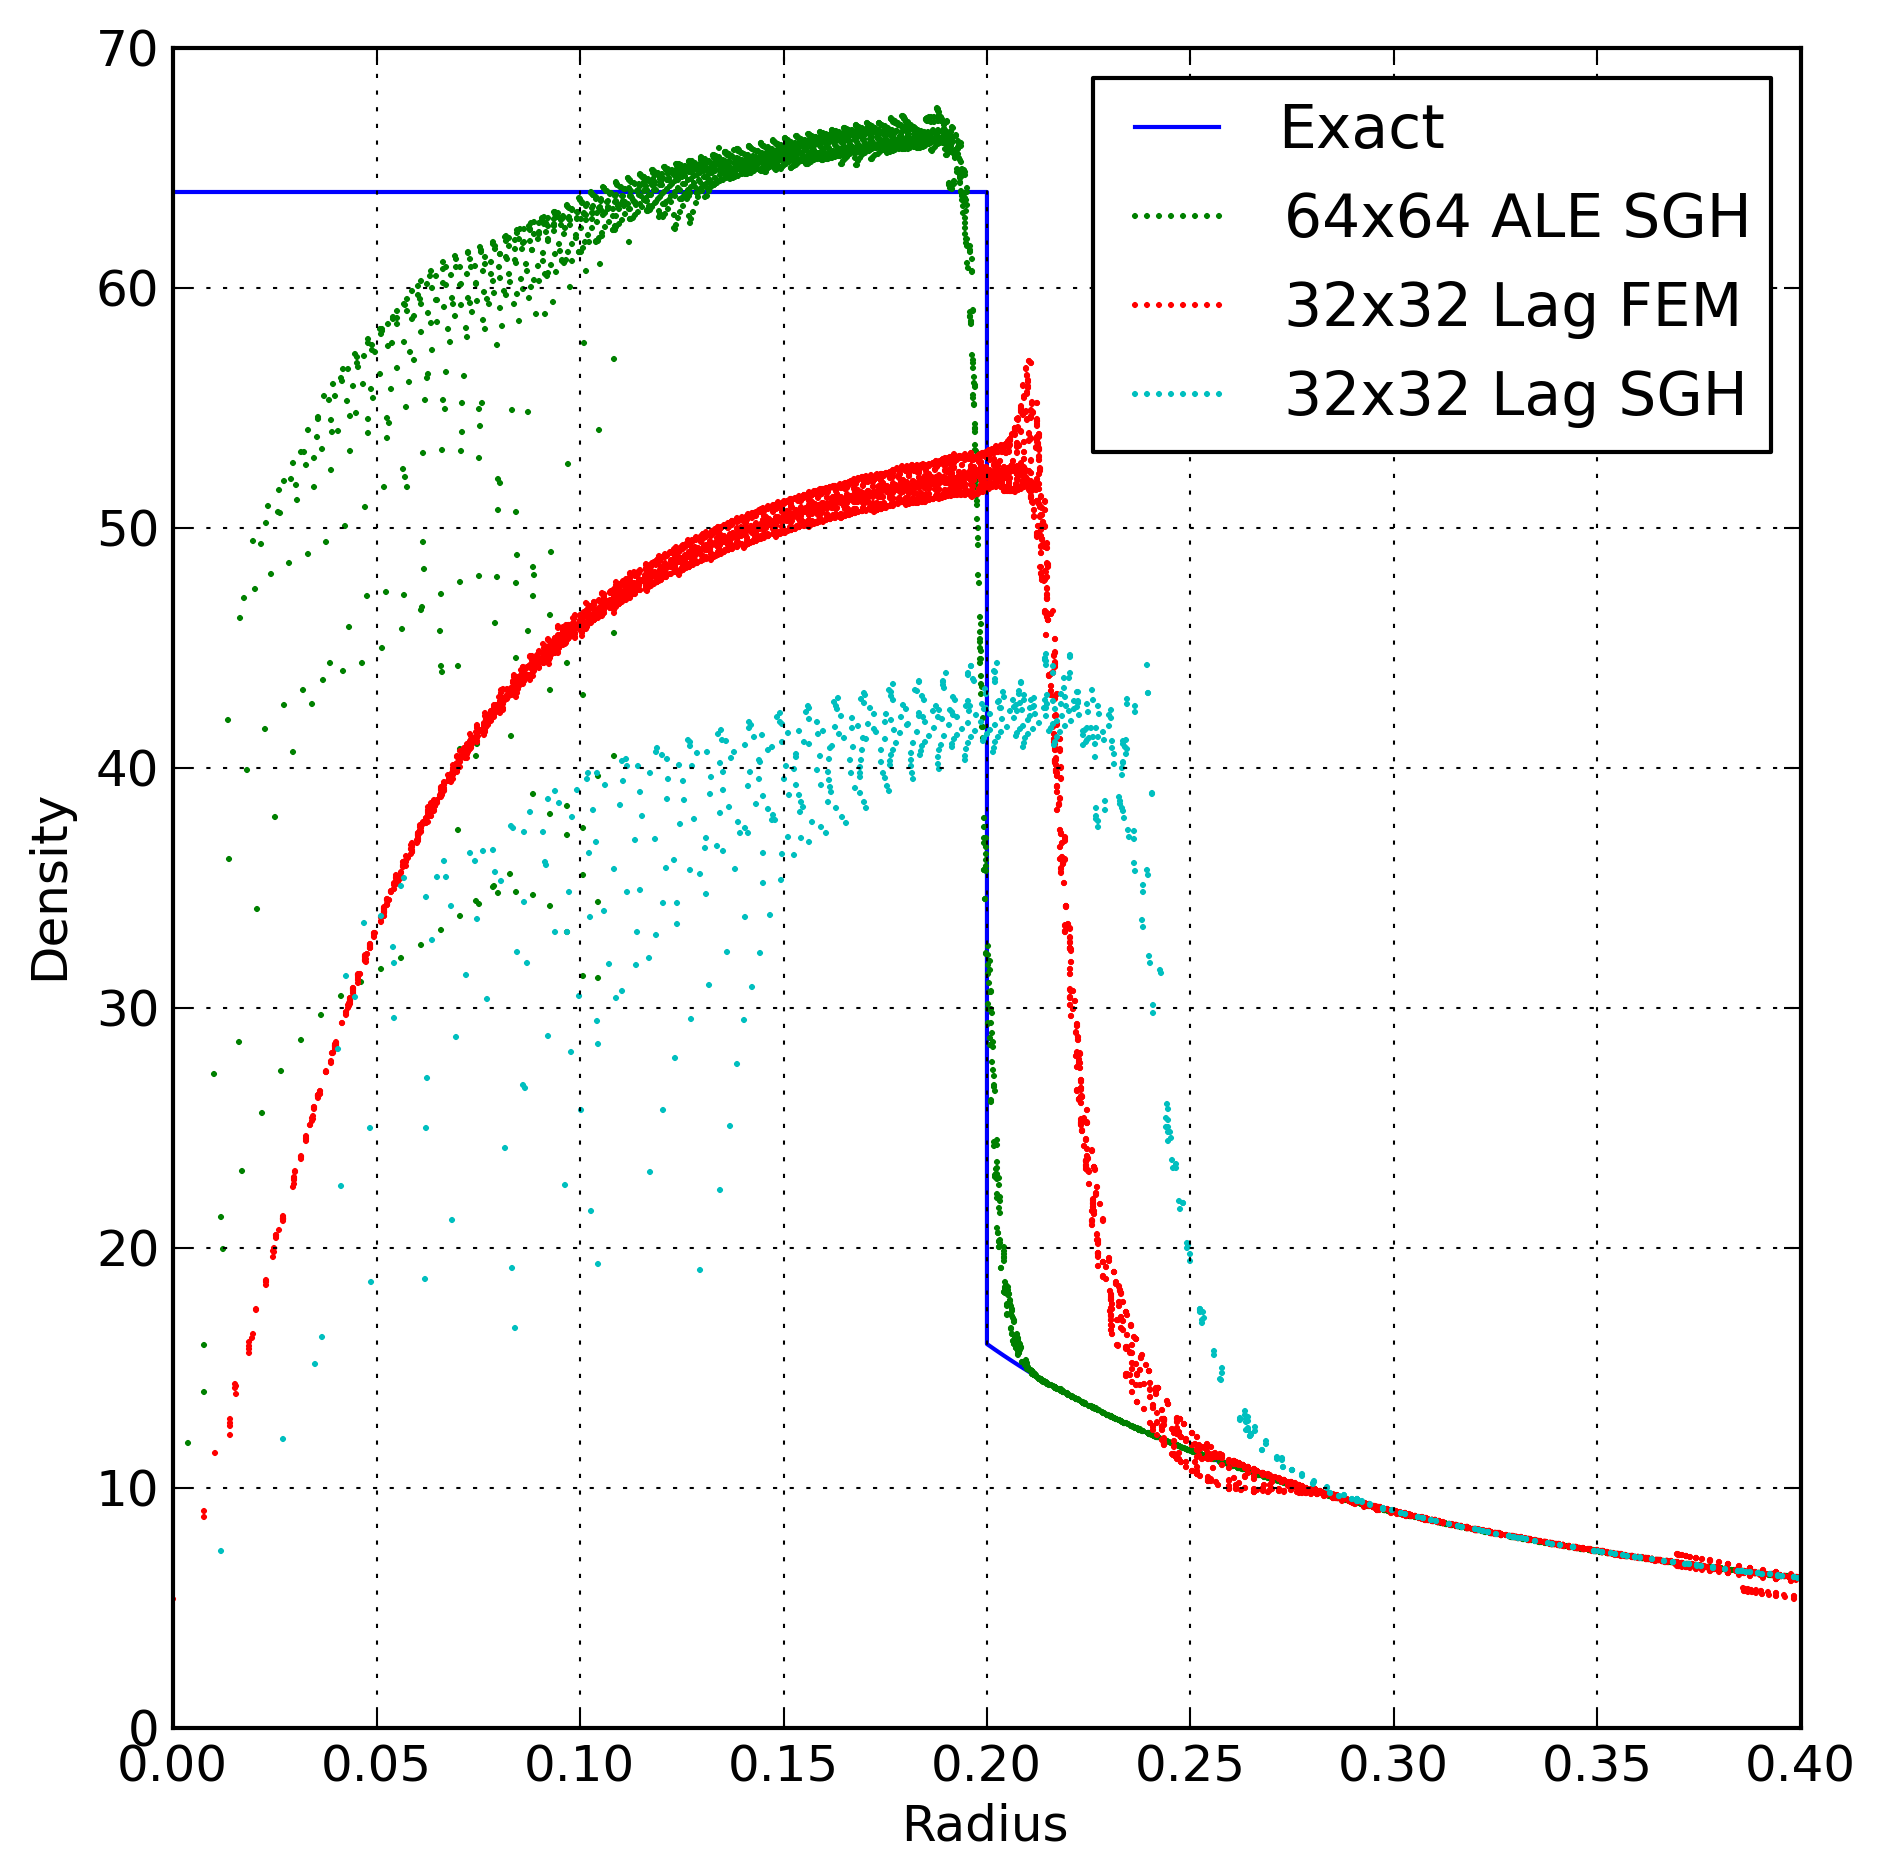
\includegraphics[width=1\textwidth]{figures/CodeComparison_Noh.png}
\vskip-2ex
\begin{itemize}
\item SGH does not preserve symmetry
\item ALE gives good shock prediction
\item FEM preserves symmetry
\end{itemize}
\end{center}
\end{column}
\begin{column}{0.5\textwidth}
\begin{center}
Lagrangian FEM Convergence
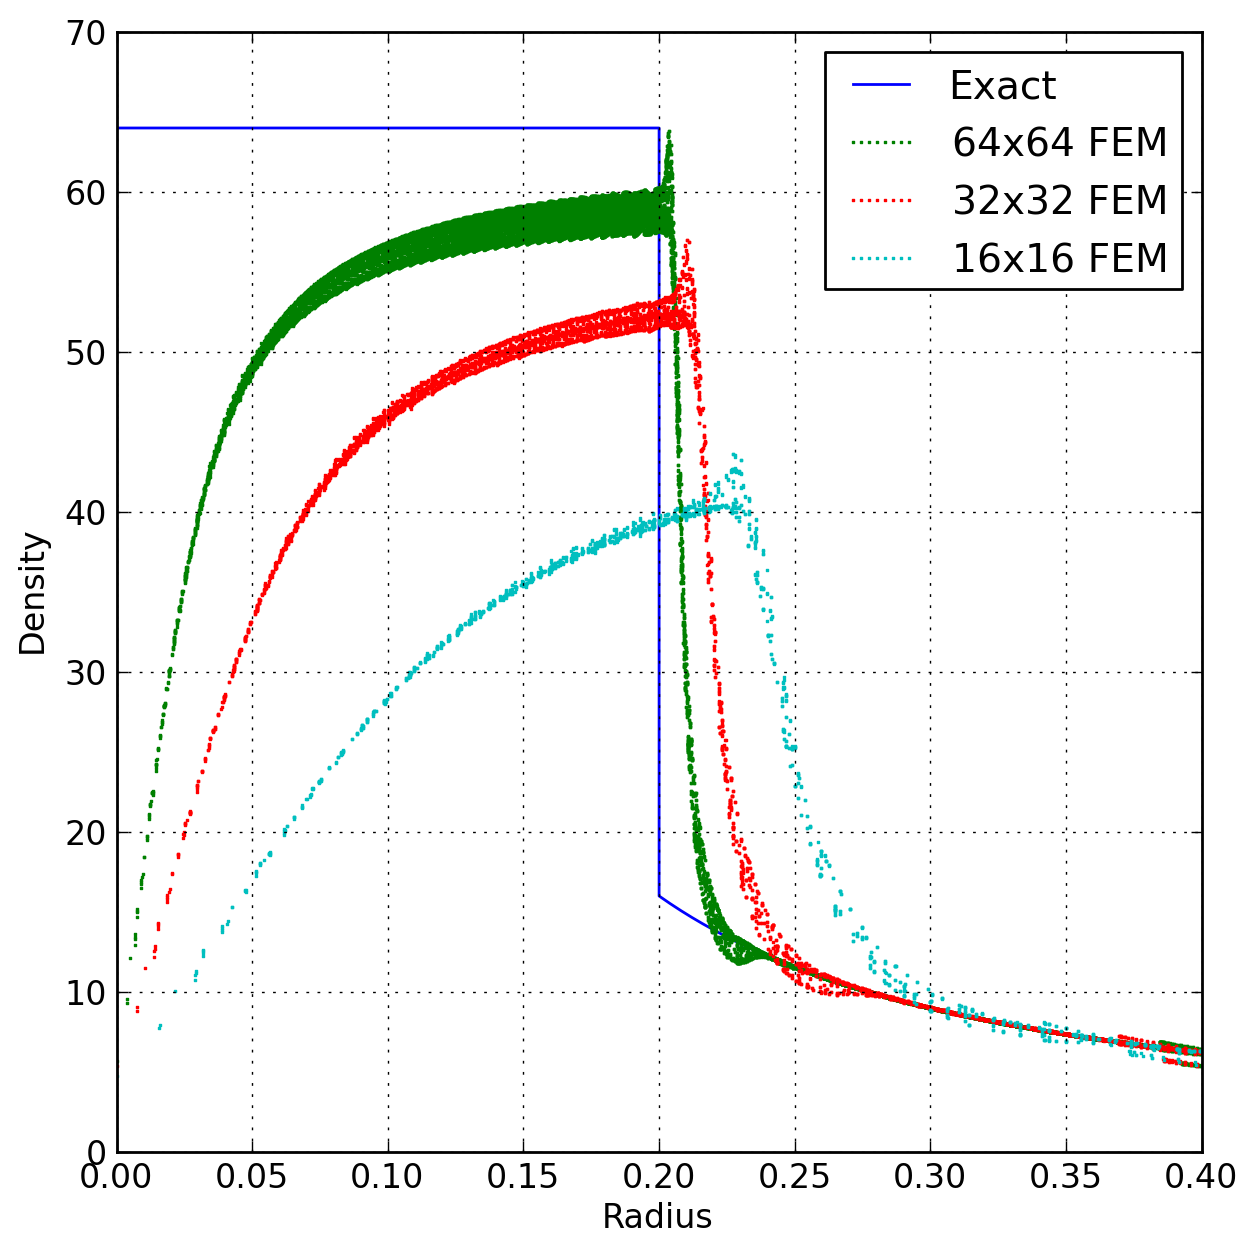
\includegraphics[width=1\textwidth]{figures/Noh_Convergence.png}
\vskip-2ex
\begin{itemize}
\item FEM converges to correct solution
\item Wall heating is typical for Lagrangian methods
\end{itemize}
\end{center}
\end{column}
\end{columns}
\end{frame}
\note{
The scatter plots reveal that the SGH simulations, whether Lagrangian or ALE,
did not preserve symmetry. ALE definitely fixed the shock prediction, and we get
an overall better result than the 32x32 Lagrangian FEM, but this is not exactly
a fair comparison. Remember that 64x64 Lagrangian SGH would not even run, and we
were forced to apply ALE. I'm sure that if we ran the FEM code with mesh
relaxation, we would get a much improved result. A completely level playing
field would be to compare the two cyan results. The 32x32 SGH and the 16x16
FEM were both run purely Lagrangian and have an equal number of DOFs.
\\ \bigskip

From the figure on the right we can see that even in pure Lagrangian mode, we
do converge to the exact solution under refinement while preserving symmetry.
}


\begin{frame}
\frametitle{Axisymmetric Noh - Energy Conservation}
\begin{columns}[T]
\begin{column}{0.5\textwidth}
\begin{center}
Comparison of Energy Conservation
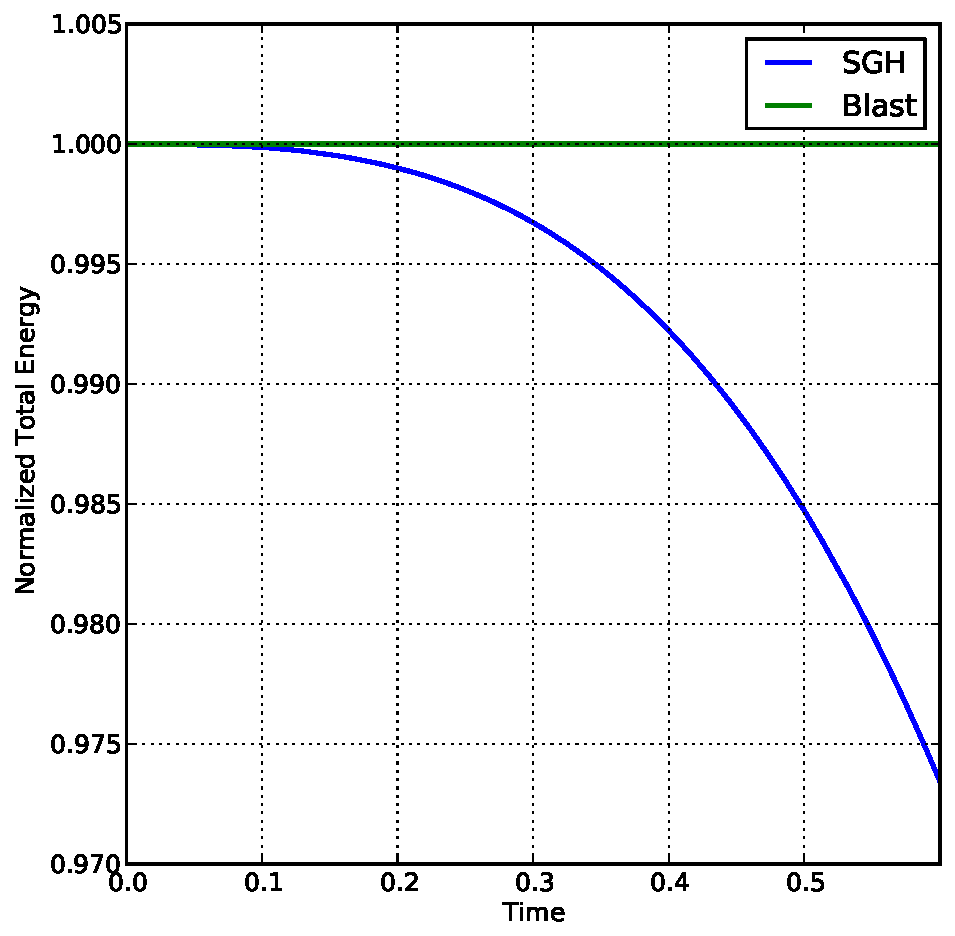
\includegraphics[width=1\textwidth]{figures/EnergyCons_Noh.pdf}
\vskip-2ex
\begin{itemize}
\item ALE SGH loses 3\% energy
\item BLAST conserves energy to machine precision
\end{itemize}
\end{center}
\end{column}
\begin{column}{0.5\textwidth}
\begin{center}
BLAST Energy Transfer
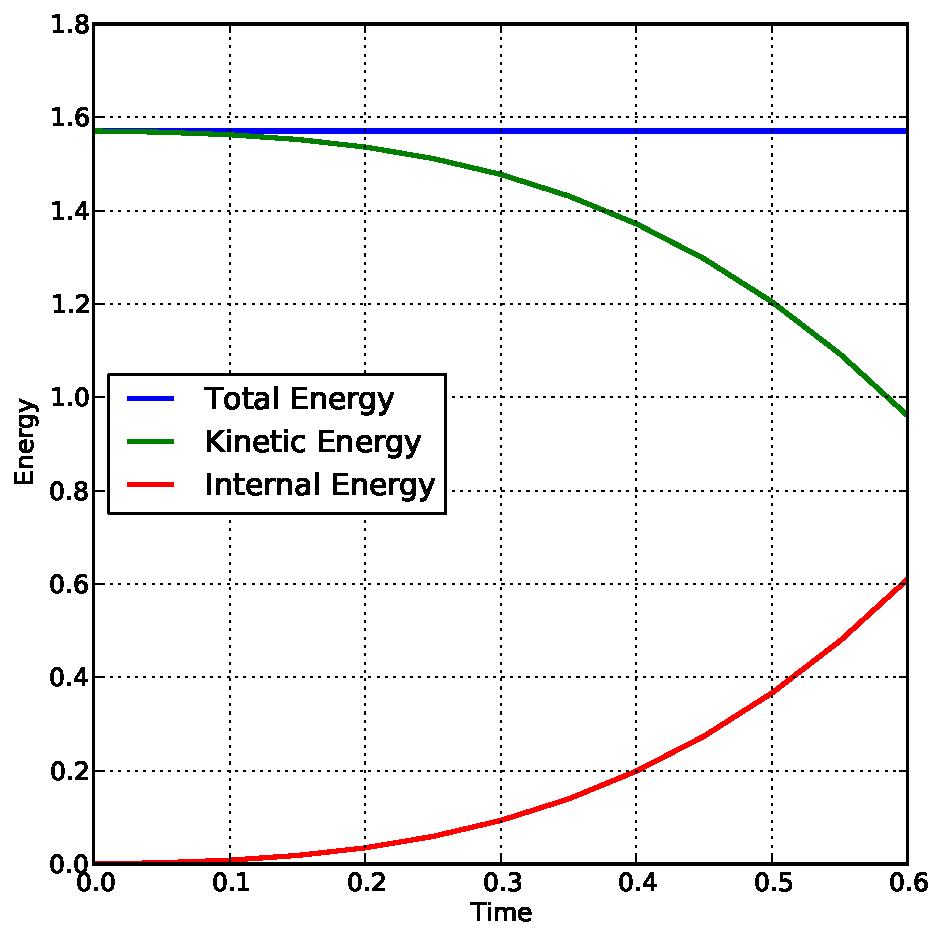
\includegraphics[width=1\textwidth]{figures/EnergyConv_Noh.pdf}
\vskip-2ex
\begin{itemize}
\item BLAST converts KE to IE without loss
\end{itemize}
\end{center}
\end{column}
\end{columns}
\end{frame}
\note{
Not only do we preserve symmetry on this difficult problem, but BLAST converts
between KE and IE without loss while SGH loses about 3\% total energy during the
simulation.
}


\subsection{Axisymmetric ICF-like Problem}


\begin{frame}
\frametitle{Simple Velocity Driven ICF-like Test}
\begin{columns}[T]
\begin{column}{0.5\textwidth}
\begin{center}
Internal Energy
\animategraphics[width=1\textwidth,every=2,final]{12}{
figures/simpleicf_vdrive/sgh_ale_energy_reflect}{0000}{0200}\\
log(Density) \\[1ex]
ALE Staggered Grid Hydro
\end{center}
\end{column}
\begin{column}{0.5\textwidth}
\begin{center}
Internal Energy
\animategraphics[width=1\textwidth,every=2,final]{12}{
figures/simpleicf_vdrive/fem_lag_energy_reflect}{0000}{0200}\\
log(Density) \\[1ex]
Pure Lagrangian FEM
\end{center}
\end{column}
\end{columns}
\end{frame}
\note{
Let's go back to the ICF-like tests we were considering earlier. Here is a minor
variant of the previous problems with a velocity drive. Let's see how ALE SGH
does on this problem.\\
(play movie)\\ \bigskip

All of those interesting flow features that we see are wrong; they are purely
numerical. This problem is supposed to be completely radial. If we were using
this as a baseline design for NIF, we would have a hard time distinguishing what
was real from what was numerical. \\ \bigskip

Now consider the same problem run with our Lagrangian FEM method. If you look at
the level lines of density, you can see that this solution remains very
symmetric. This isn't perfect, we still see some assymetries at the material
interface and near the origin, but this is much improved.
}


\subsection{Axisymmetric Triple Point Shock}


\begin{frame}\frametitle{Axisymmetric Triple Point Shock}
\begin{center}
Density
\animategraphics[width=1\textwidth,every=2,final]{12}{
figures/triple-pt_axi/triple-pt_axi_density-}{0}{193}
\end{center}
\begin{itemize}
\item More complicated shock flow
\item Multi-material Riemann problem
\item No spurious features near the axis of symmetry
\item Demonstrates robustness of higher order FEM
\end{itemize}
\end{frame}
\note{
Now we are going to switch our focus. In the previous problems we were concerned
with symmetry preservation and exact energy conservation. The following problems
will also conserve energy, but we wanted to demonstrate that the symmetry
preservation is not a cheat. There is not supposed to be any radial symmetry in
the following two problems. We also wish to demonstrate the robustness of our
method to more complicated flow geometries. \\ \bigskip

Here we have a multi-material Riemann problem. With a shock passing through the
interface of low density fluid surrounding a high density cylinder. The shock
will cause the heavy fluid to swirl into the light.\\ \bigskip

We want to point out the lack of any spurious behavior near the axis of symmetry
and that this was a purely Lagrangian calculation. Let's zoom in on the elements
in the middle of the swirl.
}


\begin{frame}\frametitle{Axisymmetric Triple Point Shock}
\begin{columns}
\begin{column}{0.3\textwidth}
\begin{itemize}
\item High aspect ratios \\[2ex]
\item Curved zones \\[2ex]
\item Impossible to represent with straight edges
\end{itemize}
\end{column}
\begin{column}{0.7\textwidth}
\begin{center}
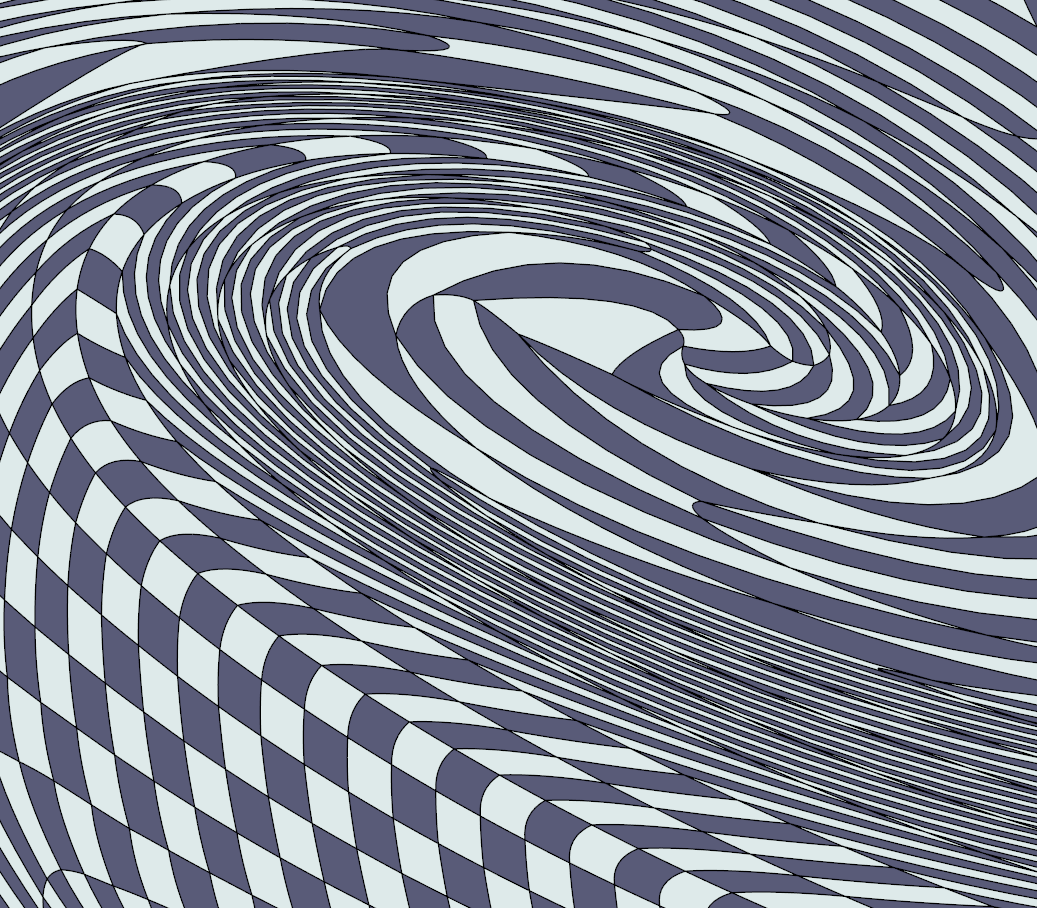
\includegraphics[height=0.8\textheight]{
figures/triple-pt_axi/triple-pt_axi_coloring_closeup.png} \\
Closeup of skewed zones in the triple point shock
\end{center}
\end{column}
\end{columns}
\end{frame}
\note{
We can see some super stretched elements and many zones with very curved edges.
This simulation would not be possible with low order straight-edged elements.
The zones would go degenerate long before this point.
}


\begin{frame}\frametitle{Axisymmetric Triple Point Shock}
\begin{center}
\animategraphics[height=0.85\textheight,every=2,final]{12}{
figures/triple-pt_axi/triple-pt_axi_density_visit-}{0}{195}
\end{center}
\end{frame}
\note{
Now let's watch a movie of the actual problem we are solving. This is just the
high density fluid as it mushrooms out into the light fluid.
}


\subsection{Axisymmetric Helium Bubble}


\begin{frame}\frametitle{Axisymmetric Helium Bubble}
\begin{center}
\animategraphics[width=1\textwidth,every=2,final]{12}{
figures/he_bubble_axi/he_bubble_axi_density-}{0}{145}
\end{center}
\begin{itemize}
\item Unstructured mesh with local refinement
\item Shock remains straight before impact
\item No spurious features near the axis of symmetry
\item Demonstrates robustness of higher order FEM
\end{itemize}
\end{frame}
\note{
This is another problem which really stresses the robustness of our method. This
is a sphere of helium that gets impacted with a shock. We have a locally refined
unstructured, curved mesh. Notice that despite the unstructured mesh, the shock
remains straight before it hits the bubble. Also note the robustness of the
elements to be able to bend and deform to make this simulation possible.
}


\begin{frame}\frametitle{Axisymmetric Helium Bubble}
\begin{columns}
\begin{column}{0.3\textwidth}
\begin{itemize}
\item High aspect ratios \\[2ex]
\item Curved zones \\[2ex]
\item Impossible to represent with straight edges
\end{itemize}
\end{column}
\begin{column}{0.7\textwidth}
\begin{center}
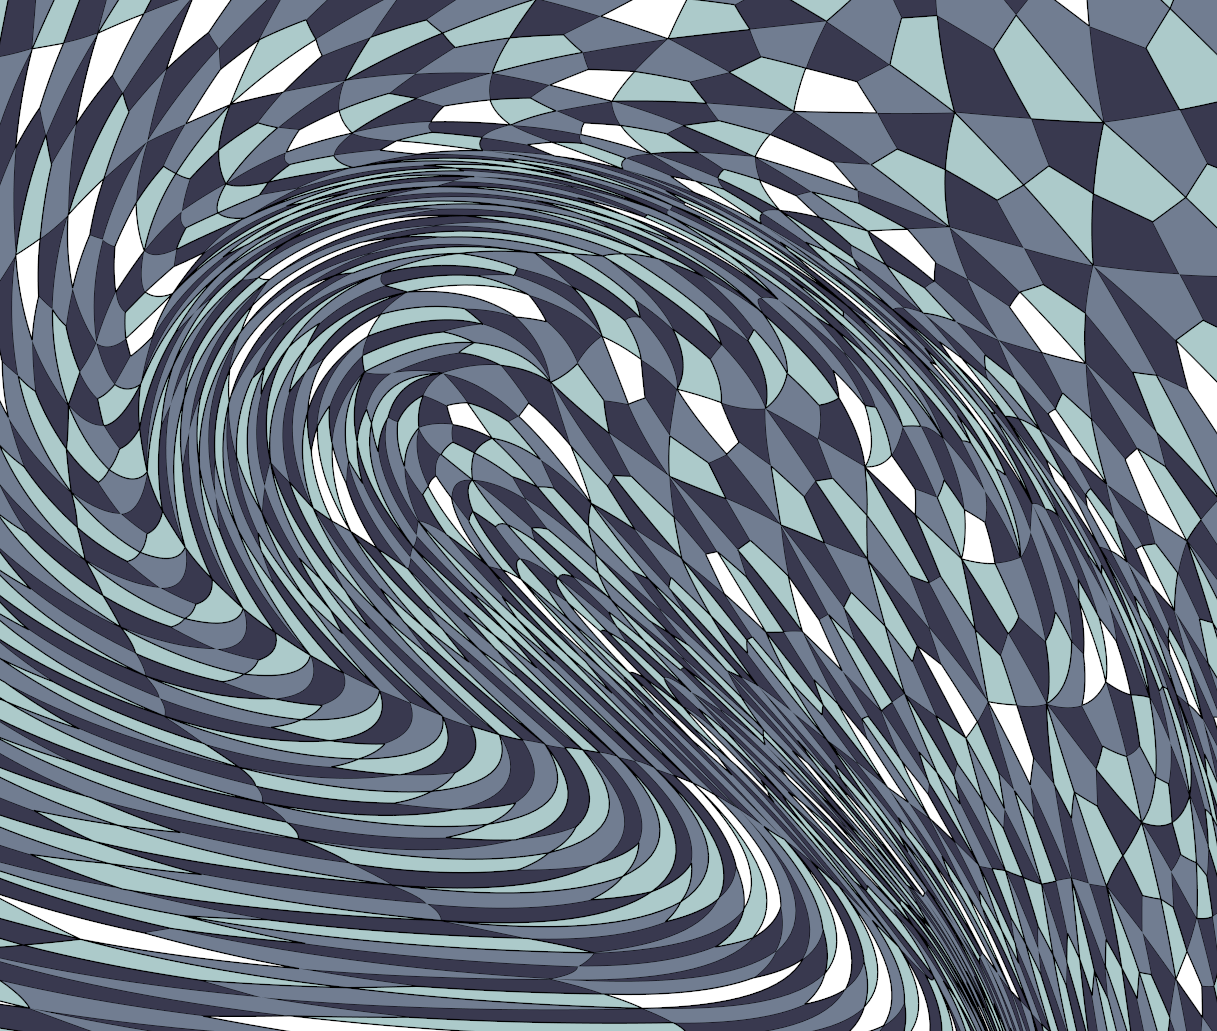
\includegraphics[height=0.75\textheight]{
figures/he_bubble_axi/he_bubble_axi_coloring_closeup.png} \\
Closeup of skewed zones in the helium bubble
\end{center}
\end{column}
\end{columns}
\end{frame}
\note{
Zooming in on the mesh, we again see many super-stretched zones, many so much so
that it is difficult to make them out. A lot more with very curved edges. Again,
this is something that would be impossible to represent and model with straight
edged elements.
}


\begin{frame}\frametitle{Axisymmetric Helium Bubble}
\begin{center}
\animategraphics[height=0.85\textheight,every=2,final]{12}{
figures/he_bubble_axi/he_bubble_axi_velocity_visit-}{0}{115}
\end{center}
\end{frame}
\note{
Here we have a video of the helium sphere turning in on itself in the process of
the simulation.
}


\subsection{Conclusions}

\begin{frame}
\frametitle{Conclusions}
We have developed a general energy-conserving, high order finite element discretization of the Euler equations in a Lagrangian frame.
\medskip

\structure{Benefits of high order elements:}
\begin{itemize}
\item The ability to more accurately capture geometrical features of a flow
region using curvilinear zones
\item Elimination of the need for ad-hoc hourglass filters
\item Sharper resolution of a shock front for a given mesh resolution
\item The ability to represent a shock within a single zone
\item Substantial reduction in mesh imprinting for
shock wave propagation not aligned with the computational mesh
\end{itemize}

\bigskip
In this talk, we have extended this method to axisymmetric problems while simultaneously conserving energy and preserving symmetry
\medskip

\structure{Our axisymmetric formulation:}
\begin{itemize}
\item Conserves energy by construction
\item Demonstrates improved symmetry preservation
\item Is robust to complicated problem geometries
\end{itemize}
\end{frame}

\end{document}
